\documentclass[a4paper,12pt]{article} 
% 使用ctex包支持中文
\usepackage[UTF8,heading = true]{ctex}
\usepackage[utf8]{inputenc}
\usepackage[T1]{fontenc}
\usepackage{graphicx}
\usepackage{float}
\usepackage{amsmath}
\usepackage{amsfonts}
\usepackage{amssymb}
\usepackage{booktabs}
\usepackage{multirow}
\usepackage{subcaption}
\usepackage{indentfirst}
\usepackage{geometry}
\usepackage{fancyhdr}
\usepackage{booktabs}
\usepackage{ctex}
\usepackage[labelfont=bf]{caption}

\geometry{left=3cm,right=3cm,top=3cm,bottom=3cm}
\usepackage{listings}
\usepackage{xcolor}



% Define VSCode style colors
\definecolor{vscodeBlue}{RGB}{97, 175, 239}
\definecolor{vscodeGreen}{RGB}{152, 195, 121}
\definecolor{vscodeRed}{RGB}{224, 108, 117}
\definecolor{vscodePurple}{RGB}{198, 120, 221}
\definecolor{vscodeGray}{RGB}{171, 178, 191}
\definecolor{vscodeBackground}{RGB}{248, 248, 255}
\definecolor{vscodeOrange}{RGB}{229, 192, 123}
\definecolor{vscodeYellow}{RGB}{229, 231, 121}
\definecolor{vscodeText}{RGB}{30, 30, 30}

\lstdefinestyle{vscode}{
	backgroundcolor=\color{vscodeBackground},
	commentstyle=\color{vscodeGray},
	keywordstyle=\color{vscodePurple},
	numberstyle=\tiny\color{vscodeGray},
	stringstyle=\color{vscodeGreen},
	basicstyle=\ttfamily\small\color{vscodeText},
	emph={LinearRegressionModel, generate_synthetic_data, train_model, evaluate_model, plot_results}, 
	emphstyle=\color{vscodeBlue},
	breakatwhitespace=false,         
	breaklines=true,                 
	captionpos=b,                    
	keepspaces=true,                 
	numbers=left,                    
	numbersep=5pt,                  
	showspaces=false,                
	showstringspaces=false,
	showtabs=false,                  
	tabsize=4,
	morekeywords={with, as, for, in, def, class, return, super, import, if, else, elif},
	keywordstyle=[2]\color{vscodeOrange},
	morekeywords=[2]{torch, nn, optim, plt, np, pd, sns, tf},
	keywordstyle=[3]\color{vscodeRed},
	morekeywords=[3]{input, output, layer, dense, activation, compile, fit, predict, evaluate},
	keywordstyle=[4]\color{vscodeYellow},
	morekeywords=[4]{int, float, str, list, dict, set, tuple, bool}
}

\lstset{style=vscode}


\ctexset{
    % 修改 section。
    section={   
        name={实验,:},
        number={\chinese{section}},
        format=\heiti\bfseries\centering\zihao{-2} % 设置 section 标题为黑体、右对齐、小4号字
    },
    % 修改 subsection。
    subsection={   
        name={,、},
        number={\chinese{subsection}},
        format=\songti\bfseries\zihao{4} % 设置 subsection 标题为黑体、5号字
    },
    % 修改 subsection。
    subsubsection={   
        name={,、},
        number={\arabic{subsubsection}},
        format=\songti\bfseries\zihao{-4} % 设置 subsection 标题为黑体、5号字
    }
}
\fancyhead{}


\begin{document}

%制作封面
\begin{titlepage}
    \begin{center}
        \par
            \centerline{
\includegraphics[scale=1.5]{data/media/image1.jpeg} 
\includegraphics[scale=3]{data/media/image2.jpeg}} %插入图片
        \par
		\vskip 5cm
		\lishu \fontsize{50}{20} 实\quad 验\quad 报\quad 告
		\vskip 10cm

	\begin{center}
		\begin{tabular}{l}
		\songti \zihao{-2} \bfseries 课程名称:深度学习与计算机视觉实验
		\quad \\
	    	\songti \zihao{-2} \bfseries 学生姓名:刘兴琰
	    	\quad \\
		\songti \zihao{-2} \bfseries 学生学号:		202264690069          
		\quad \\
	    	\songti \zihao{-2} \bfseries 学生专业:		人工智能     
	    	\quad \\
	     \songti \zihao{-2} \bfseries 开课学期 :		2024年大二学年第二学期    
	     \quad \\
           \songti \zihao{-2} \bfseries  提交日期:\quad 2024年\quad 5  月\quad 7  日
    \end{tabular}
	\end{center}
    \end{center}
\end{titlepage}


% 生成目录
\newpage
\pagestyle{empty}
\begin{center}
\tableofcontents
\end{center}

\newpage

\setcounter{page}{1}

\section{线性回归模型}
\subsection{实验目的}
本实验在设计并定义一个简单的线性回归模型,以便模型能够读取数据并进行训练。通过该实验,我们希望达到以下目的:
\begin{enumerate}
	\item 掌握如何使用PyTorch定义线性回归模型;
	\item 学习如何生成合成数据进行训练和测试;
	\item 掌握如何训练模型并评估模型性能;
	\item 了解如何使用图像展示训练过程中的损失以及模型的预测效果。
\end{enumerate}

\subsection{实验原理}
在线性回归(Linear Regression)模型中,我们通过一个线性函数来描述输入变量 \(\mathbf{X}\) 与输出变量 \(y\) 之间的关系。我们假设存在这样的一个线性模型:

\[
\boxed{
	y = \mathbf{X} \mathbf{w} + \mathbf{b} + \epsilon
}
\]

其中,\(\mathbf{w}\) 是权重向量,\(\mathbf{b}\) 是偏置项,\(\epsilon\) 是随机误差。我们的目标是估计 \(\mathbf{w}\) 和 \(\mathbf{b}\) 的最佳值,使得模型对给定数据的预测误差最小。

为了实现这一目标,我们可以使用均方误差(MSE)作为损失函数。均方误差定义为:

\[
\boxed{
	\mathrm{MSE} = \frac{1}{n} \sum_{i=1}^n \left(y_i - \hat{y}_i\right)^2
}
\]

其中,\(y_i\) 是实际输出,\(\hat{y}_i\) 是预测输出,\(n\) 是样本数量。

我们希望通过最小化均方误差来估计参数 \(\mathbf{w}\) 和 \(\mathbf{b}\)。在深度学习的框架下,我们采用随机梯度下降(SGD)算法来优化模型参数。梯度下降算法通过以下步骤更新参数:

\[
\boxed{
	\mathbf{w} \leftarrow \mathbf{w} - \eta \cdot \frac{\partial \mathrm{MSE}}{\partial \mathbf{w}}
}
\]
\[
\boxed{
	\mathbf{b} \leftarrow \mathbf{b} - \eta \cdot \frac{\partial \mathrm{MSE}}{\partial \mathbf{b}}
}
\]

其中,\(\eta\) 是学习率。我们可以计算损失函数相对于参数的梯度:

\[
\boxed{
	\frac{\partial \mathrm{MSE}}{\partial \mathbf{w}} = -\frac{2}{n} \mathbf{X}^\top (\mathbf{y} - \hat{\mathbf{y}})
}
\]
\[
\boxed{
	\frac{\partial \mathrm{MSE}}{\partial \mathbf{b}} = -\frac{2}{n} \sum_{i=1}^n (y_i - \hat{y}_i)
}
\]

在训练过程中,我们通过多次迭代上述参数更新过程,直到损失函数收敛或达到预定的迭代次数。

\subsection{实验内容}
\begin{lstlisting}[language=Python, caption=线性回归Python代码]
import torch
import torch.nn as nn
import torch.optim as optim
import matplotlib.pyplot as plt
import numpy as np

class LinearRegressionModel(nn.Module):
	def __init__(self, input_dim):
		super(LinearRegressionModel, self).__init__()
		self.linear = nn.Linear(input_dim, 1)

	def forward(self, x):
		return self.linear(x)

def generate_synthetic_data(n_samples, weight, bias, noise_std):
	"""
	Generate synthetic data.

	Parameters:
	n_samples (int): number of samples.
	weight (float): weight of linear model.
	bias (float): bias of linear model.
	noise_std (float): standard deviation of noise.

	Returns:
	(Tensor, Tensor): Returns input features and target values.
	"""
	X = torch.randn(n_samples, 1)
	noise = torch.randn(n_samples, 1) * noise_std
	y = weight * X + bias + noise
	return X, y

def train_model(model, X_train, y_train, learning_rate, n_epochs):
	"""
	Train a linear regression model.

	Parameters:
	model (nn.Module): Linear regression model.
	X_train (Tensor): Training set input features.
	y_train (Tensor): Training set target value.
	learning_rate (float): Learning rate.
	n_epochs (int): Number of training rounds.

	Returns:
	list: Training loss for each epoch.
	"""
	
	criterion = nn.MSELoss()
	optimizer = optim.SGD(model.parameters(), lr=learning_rate)
	losses = []

	for epoch in range(n_epochs):
		model.train()
		optimizer.zero_grad()
		y_pred = model(X_train)
		loss = criterion(y_pred, y_train)
		loss.backward()
		optimizer.step()
		losses.append(loss.item())

	return losses

def evaluate_model(model, X_test, y_test):
	"""
	Evaluate a linear regression model.

	Parameters:
	model (nn.Module): Linear regression model.
	X_test (Tensor): Test set input features.
	y_test (Tensor): Test set target values.

	Returns:
	(float, Tensor): Returns the mean squared error and predicted values.
	"""
	model.eval()
	with torch.no_grad():
	y_pred = model(X_test)
	mse = nn.MSELoss()(y_pred, y_test)
	return mse.item(), y_pred

def plot_results(losses, X_test, y_test, y_pred):
	"""
	Plot the training loss and the comparison of actual value and predicted value.
	
	Parameters:
	losses (list): training loss.
	X_test (Tensor): test set input features.
	y_test (Tensor): test set target value.
	y_pred (Tensor): test set predicted value.
	"""
	plt.figure(figsize=(14, 5))

	plt.subplot(1, 2, 1)
	plt.plot(losses)
	plt.title("Training Loss over Epochs")
	plt.xlabel("Epochs")
	plt.ylabel("Loss")

	plt.subplot(1, 2, 2)
	plt.scatter(X_test, y_test, label="Actual")
	plt.scatter(X_test, y_pred, label="Predicted")
	plt.title("Actual vs Predicted")
	plt.xlabel("X values")
	plt.ylabel("Y values")
	plt.legend()
	plt.show()
	
# Data generation and model training
n_samples = 1000
weight = 2.0
bias = 1.0
noise_std = 0.1
learning_rate = 0.01
n_epochs = 100

X, y = generate_synthetic_data(n_samples, weight, bias, noise_std)

X_train, X_test = X[:80], X[80:]
y_train, y_test = y[:80], y[80:]

input_dim = X_train.shape[1]
model = LinearRegressionModel(input_dim)

losses = train_model(model, X_train, y_train, learning_rate, n_epochs)

mse, y_pred = evaluate_model(model, X_test, y_test)

plot_results(losses, X_test, y_test, y_pred)
\end{lstlisting}

\subsection{实验结果}
\begin{figure}[htbp]
	\centering
	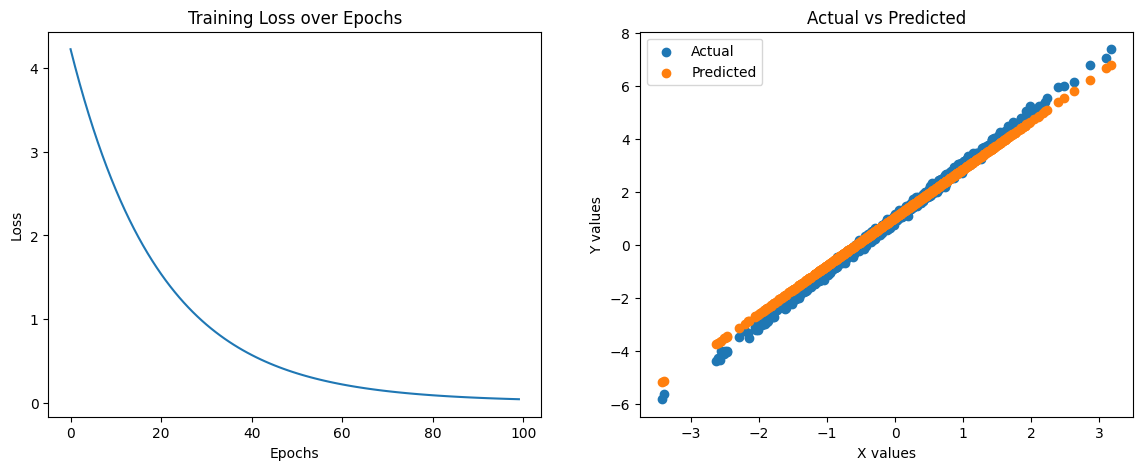
\includegraphics[width=1\textwidth]{1.png}
	\caption{线性回归结果图}
\end{figure}
在这个简单的数据集中,线性回归展现了良好的性能,同时收敛结果比较理想。



\section{softmax回归模型}
\subsection{实验目的}
	在本实验中,我们设计了一个 Softmax 回归模型进行 Fashion-MNIST数据集的多分类任务。Fashion-MNIST 数据集包含 10 类物品,每类包含 6,000 张训练图片和 1,000 张测试图片。每张图片的尺寸为 $28 \times 28$ 像素,并以 0-9 的整数标签表示类别。

\subsection{实验原理}
\subsubsection{Softmax回归模型}
Softmax 回归模型是一种线性模型,它的目标是最大化样本属于每个类别的概率。该模型可以表示为:

\begin{equation}
	\hat{y} = \text{softmax}(XW + b)
\end{equation}

其中:
\begin{itemize}
	\item $X$ 为输入数据矩阵,形状为 $n \times d$,其中 $n$ 为样本数,$d$ 为特征数;
	\item $W$ 为权重矩阵,形状为 $d \times k$,其中 $k$ 为类别数;
	\item $b$ 为偏置向量,形状为 $1 \times k$;
	\item $\hat{y}$ 为输出概率分布,形状为 $n \times k$。
\end{itemize}

Softmax 函数定义为:

\begin{equation}
	\text{softmax}(z_i) = \frac{e^{z_i}}{\sum_{j=1}^k e^{z_j}}
\end{equation}

其中 $z = XW + b$。

\subsubsection{损失函数}
我们使用交叉熵损失函数来评估模型的性能:

\begin{equation}
	\text{CrossEntropyLoss} = -\sum_{i=1}^n \sum_{j=1}^k y_{ij} \log(\hat{y}_{ij})
\end{equation}

其中 $y_{ij}$ 为样本 $i$ 属于类别 $j$ 的指示符。

\subsubsection{优化方法}
为了最小化交叉熵损失,我们使用梯度下降法来更新参数:

\begin{equation}
	W_{t+1} = W_t - \eta \cdot \frac{\partial \text{CrossEntropyLoss}}{\partial W} \\
\end{equation}

\begin{equation}
	b_{t+1} = b_t - \eta \cdot \frac{\partial \text{CrossEntropyLoss}}{\partial b}
\end{equation}

其中 $\eta$ 为学习率。



\subsection{实验内容}
\begin{enumerate}
	\item \textbf{数据预处理}:
	\begin{itemize}
		\item \textbf{图像展平}:将 Fashion-MNIST 数据集的图像数据展平为一维向量。
		\item \textbf{归一化}:将像素值归一化至 $[0, 1]$ 区间。
	\end{itemize}
	
	\item \textbf{构建模型}:
	\begin{itemize}
		\item 初始化权重矩阵 $W$ 和偏置向量 $b$。
		\item \textbf{正则化}:添加正则化项 $\frac{\lambda}{2} \|W\|^2$ 来控制模型的复杂度,其中 $\lambda$ 为正则化系数。
	\end{itemize}
	
	\item \textbf{训练模型}:
	\begin{itemize}
		\item \textbf{前向传播}:计算线性组合 $z = XW + b$。
		\item \textbf{Softmax}:通过 Softmax 函数 $\hat{y} = \text{softmax}(z)$ 将其转换为概率分布。
		\item \textbf{损失计算}:计算交叉熵损失 $L = -\sum_{i=1}^n \sum_{j=1}^k y_{ij} \log(\hat{y}_{ij})$。
		\item \textbf{反向传播}:计算损失对 $W$ 和 $b$ 的导数,更新模型参数。
	\end{itemize}
	
	\item \textbf{测试模型}:
	\begin{itemize}
		\item 使用测试集评估模型性能。
		\item 计算模型的准确率 $Accuracy = \frac{1}{n} \sum_{i=1}^n \delta(\arg\max(\hat{y}_i), y_i)$,其中 $\delta$ 是克罗内克尔函数。
	\end{itemize}
\end{enumerate}
\begin{lstlisting}[language=Python, caption=Softmax回归模型Python代码]
import tensorflow as tf
import numpy as np
import matplotlib.pyplot as plt
import seaborn as sns
from sklearn.metrics import classification_report, confusion_matrix

def load_and_prepare_data():
	(x_train, y_train), (x_test, y_test) = tf.keras.datasets.fashion_mnist.load_data()
	x_train, x_test = x_train / 255.0, x_test / 255.0  

	x_train = x_train[..., np.newaxis]
	x_test = x_test[..., np.newaxis]
	return x_train, y_train, x_test, y_test

def build_model():
	model = tf.keras.Sequential([
		tf.keras.layers.Flatten(input_shape=(28, 28, 1)),
		tf.keras.layers.Dense(10, activation='softmax')
	])
	model.compile(optimizer='adam',
		loss='sparse_categorical_crossentropy',
		metrics=['accuracy'])
	return model

def train_model(model, x_train, y_train):
	history = model.fit(x_train, y_train, epochs=10, validation_split=0.2, verbose=2)
	return history

def evaluate_model(model, x_test, y_test):
	test_loss, test_accuracy = model.evaluate(x_test, y_test, verbose=2)
	y_pred = np.argmax(model.predict(x_test), axis=1)
	return test_loss, test_accuracy, y_pred

def plot_training_history(history):
	plt.figure(figsize=(12, 5))

	plt.subplot(1, 2, 1)
	plt.plot(history.history['accuracy'], label='Train Accuracy')
	plt.plot(history.history['val_accuracy'], label='Val Accuracy')
	plt.xlabel('Epoch')
	plt.ylabel('Accuracy')
	plt.title('Training and Validation Accuracy')
	plt.legend()

	plt.subplot(1, 2, 2)
	plt.plot(history.history['loss'], label='Train Loss')
	plt.plot(history.history['val_loss'], label='Val Loss')
	plt.xlabel('Epoch')
	plt.ylabel('Loss')
	plt.title('Training and Validation Loss')
	plt.legend()

	plt.tight_layout()
	plt.show()

def plot_classification_report(y_test, y_pred):
	print(classification_report(y_test, y_pred, target_names=[
		'T-shirt/top', 'Trouser', 'Pullover', 'Dress', 'Coat',
		'Sandal', 'Shirt', 'Sneaker', 'Bag', 'Ankle boot']))

def plot_confusion_matrix(y_test, y_pred):
	cm = confusion_matrix(y_test, y_pred)
	plt.figure(figsize=(10, 8))
	sns.heatmap(cm, annot=True, fmt='d', cmap='Blues', xticklabels=[
		'T-shirt/top', 'Trouser', 'Pullover', 'Dress', 'Coat',
		'Sandal', 'Shirt', 'Sneaker', 'Bag', 'Ankle boot'],
	yticklabels=[
		'T-shirt/top', 'Trouser', 'Pullover', 'Dress', 'Coat',
		'Sandal', 'Shirt', 'Sneaker', 'Bag', 'Ankle boot'])
	plt.xlabel('Predicted Label')
	plt.ylabel('True Label')
	plt.title('Confusion Matrix')
	plt.show()

def plot_example_predictions(x_test, y_test, y_pred):
	plt.figure(figsize=(10, 10))
	for i in range(9):
		plt.subplot(3, 3, i + 1)
		plt.imshow(x_test[i].reshape(28, 28), cmap='gray')
		plt.title(f"Pred: {y_pred[i]}, Actual: {y_test[i]}")
		plt.axis('off')
	plt.tight_layout()
	plt.show()


x_train, y_train, x_test, y_test = load_and_prepare_data()


model = build_model()


history = train_model(model, x_train, y_train)


test_loss, test_accuracy, y_pred = evaluate_model(model, x_test, y_test)


plot_training_history(history)
plot_classification_report(y_test, y_pred)
plot_confusion_matrix(y_test, y_pred)
plot_example_predictions(x_test, y_test, y_pred)
\end{lstlisting}


\subsection{实验结果}
该模型的训练数据集为时尚物品分类数据集Fashion MNIST,它包含10个类别的服装和鞋类图像。每个类别包含1000个图像,总共有10,000个测试图像。

训练过程中,我们发现模型在训练和验证数据上的损失和准确性逐渐趋于稳定。经过10个周期的训练后,模型在测试集上的准确性为0.8432。通过观察分类报告,可以看出模型在不同类别上的表现有所不同。

从混淆矩阵得出以下几点:
模型在不同类别上的精确度有所差异。
裤子(Trouser)、凉鞋(Sandal)和包(Bag)的精确度相对较高,达到了93% 
以上,而衬衫(Shirt)的精确度较低,为0.66。模型对大多数类别的召回率都较高,尤其是对裤子(Trouser)和凉鞋(Sandal)的召回率接近1。但对衬衫(Shirt)的召回率只有0.51,表明模型对衬衫的分类存在较大的误差。F1分数是精确度和召回率的调和平均值,是衡量模型性能的重要指标。大多数类别的F1分数都在0.70以上,表明模型总体表现良好,但在衬衫(Shirt)和毛衣(Pullover)等类别上表现相对较差。
\begin{figure}[htbp]
	\centering
	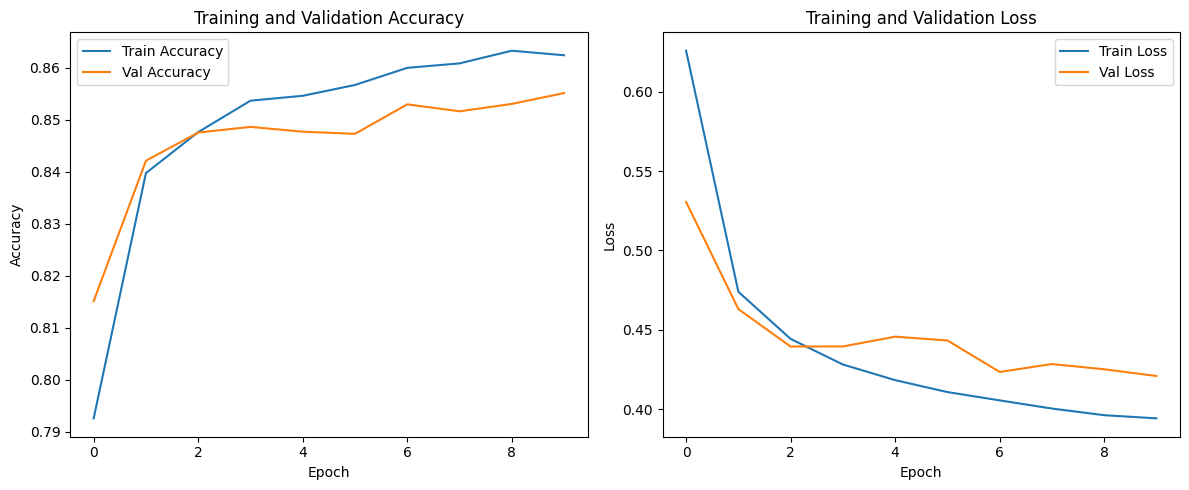
\includegraphics[width=0.8\textwidth]{2.png}
	\caption{Softmax回归训练图}
\end{figure}

\begin{figure}[htbp]
	\centering
	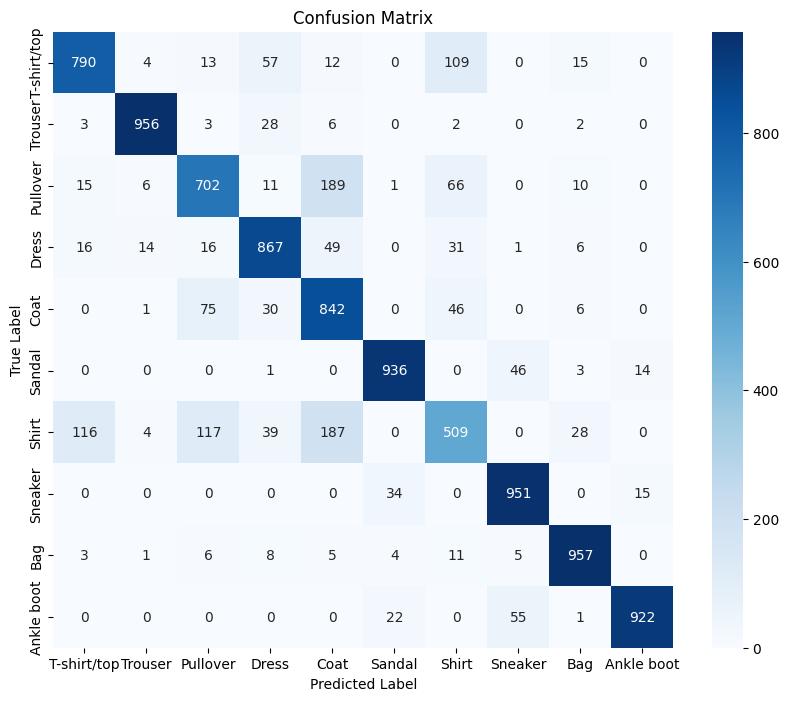
\includegraphics[width=0.6\textwidth]{3.png}
	\caption{Softmax回归训练混淆矩阵}
\end{figure}

\begin{figure}[htbp]
	\centering
	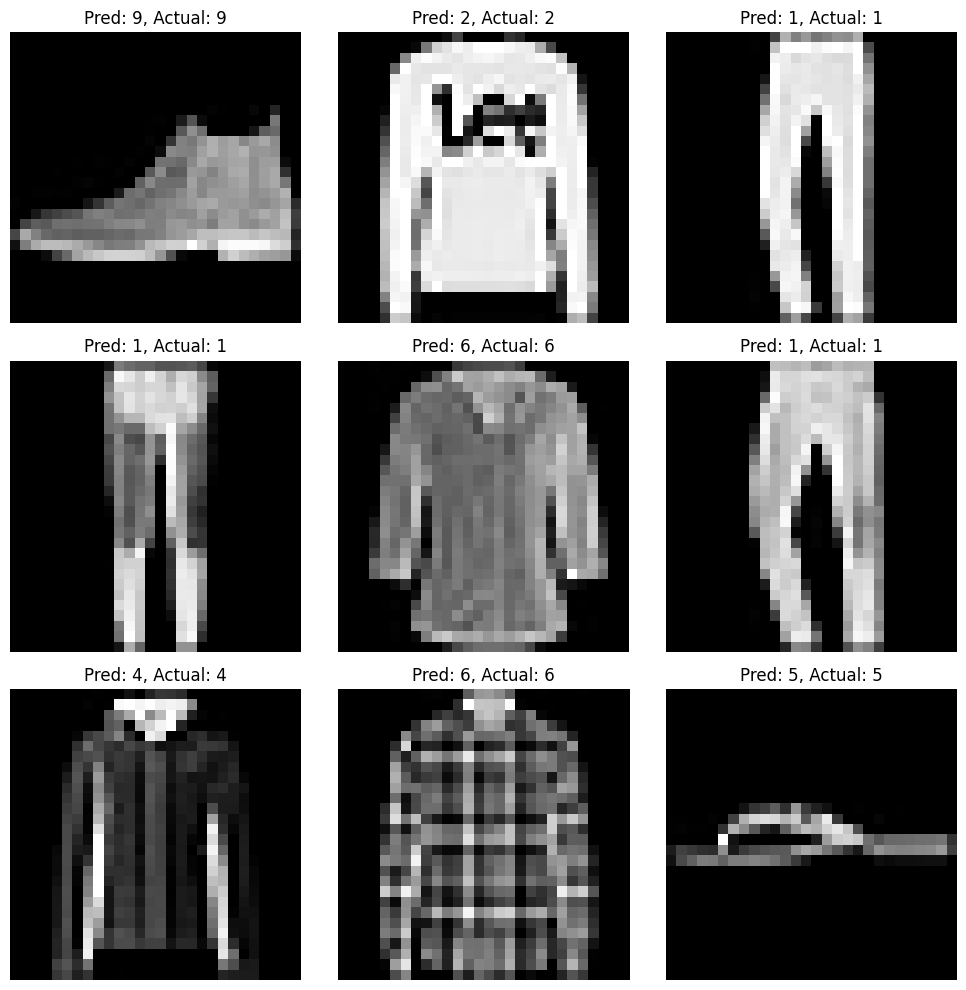
\includegraphics[width=0.6\textwidth]{4.png}
	\caption{Softmax回归结果图}
\end{figure}



\section{多层感知机模型}
\subsection{实验目的}
在本实验中,我们设计了一个 多层感知机模型进行 Fashion-MNIST数据集的多分类任务。

\subsection{实验原理}
我们设计的多层感知机(MLP)模型旨在处理Fashion-MNIST数据集上的多类分类任务。Fashion-MNIST是一个广泛使用的服装图像数据集,包含$10$个类别,如T恤、裤子、鞋等。每个图像都是$28 \times 28$像素的灰度图。

多层感知机模型是一个前馈神经网络,包含输入层、若干隐藏层和输出层。每层由多个神经元组成,每个神经元通过激活函数处理输入信号。


设输入层具有$784$个神经元(对应于$28 \times 28$像素的图像展开成的向量)。我们可以设置若干隐藏层,每层有不同数量的神经元,并选择ReLU作为激活函数,因其计算效率高且能减少梯度消失问题。输出层具有$10$个神经元,对应于10个类别,使用softmax激活函数,以输出每个类别的概率。

给定输入向量$\mathbf{x} \in \mathbb{R}^{784}$,隐藏层的输出$\mathbf{h}$可以表达为:
\[
\mathbf{h} = \sigma(\mathbf{W}_h \mathbf{x} + \mathbf{b}_h)
\]
其中,$\mathbf{W}_h$和$\mathbf{b}_h$分别是隐藏层的权重矩阵和偏置向量,$\sigma$表示ReLU激活函数。

输出层的输出$\mathbf{y}$由下式给出:
\[
\mathbf{y} = \text{softmax}(\mathbf{W}_o \mathbf{h} + \mathbf{b}_o)
\]
其中,$\mathbf{W}_o$和$\mathbf{b}_o$是输出层的权重矩阵和偏置向量。softmax函数确保输出向量$\mathbf{y}$的各分量和为1,每个分量表示相应类别的预测概率。


模型训练通过最小化交叉熵损失函数进行,该函数衡量真实标签和预测概率分布之间的差异。采用反向传播算法自动计算所需的梯度,并使用Adam优化器来更新网络参数,以提高分类准确性。


\subsection{实验内容}
\subsubsection{背景介绍}

在这次实验中,我们将使用 \texttt{Fashion MNIST} 数据集来训练一个简单的多层感知器(MLP)模型来进行图像分类。 \texttt{Fashion MNIST} 数据集是一个常用的图像分类数据集,包含10类时尚物品,每类包含7000个样本。

\subsubsection{数据准备}

数据来自 \texttt{tf.keras.datasets} 中的 \texttt{fashion\_mnist} 数据集。原始数据集中包含训练集和测试集。训练集包含60000个样本,测试集包含10000个样本。每个样本是28x28的灰度图像,表示从0到255的像素值。我们将其归一化为\[0, 1\]范围内的浮点数:

\[
x_{\text{norm}} = \frac{x}{255}
\]

对于卷积神经网络,我们还需要为每个图像添加一个通道维度。这样,图像的形状将从 (28, 28) 变为 (28, 28, 1)。

\begin{lstlisting}[language=Python]
	(x_train, y_train), (x_test, y_test) = tf.keras.datasets.fashion_mnist.load_data()
	x_train, x_test = x_train / 255.0, x_test / 255.0  
	
	x_train = x_train[..., np.newaxis]
	x_test = x_test[..., np.newaxis]
\end{lstlisting}

\subsubsection{模型构建}

我们的模型是一个简单的多层感知器(MLP),包含以下层:

\begin{enumerate}
	\item \texttt{Flatten} 层:将输入图像展平为一维向量。
	\item \texttt{Dense} 层:全连接层,输出10个类别,使用 \texttt{softmax} 激活函数。
\end{enumerate}

模型使用的损失函数为 \texttt{sparse\_categorical\_crossentropy},优化器为 \texttt{adam},评估指标为 \texttt{accuracy}:

\begin{lstlisting}[language=Python]
	model = tf.keras.Sequential([
	tf.keras.layers.Flatten(input_shape=(28, 28, 1)),
	tf.keras.layers.Dense(10, activation='softmax')
	])
	model.compile(optimizer='adam',
	loss='sparse_categorical_crossentropy',
	metrics=['accuracy'])
\end{lstlisting}

\subsubsection{模型训练}

模型训练使用训练集数据的80\%进行训练,20\%用于验证。我们训练了10个周期:

\begin{lstlisting}[language=Python]
	history = model.fit(x_train, y_train, epochs=10, validation_split=0.2, verbose=2)
\end{lstlisting}

\subsubsection{模型评估}

模型评估使用测试集。首先,我们计算模型在测试集上的损失和准确性:

\begin{lstlisting}[language=Python]
	test_loss, test_accuracy = model.evaluate(x_test, y_test, verbose=2)
\end{lstlisting}

然后,我们使用模型对测试集进行预测,并选择每个样本的预测概率最大的类别作为最终预测结果:

\begin{lstlisting}[language=Python]
	y_pred = np.argmax(model.predict(x_test), axis=1)
\end{lstlisting}
\subsection{实验结果}

\subsubsection{结果展示}


我们首先展示训练和验证的准确性以及损失随时间变化的趋势。通过绘制折线图,我们可以观察到模型训练的性能。

\begin{lstlisting}[language=Python]
	plt.figure(figsize=(12, 5))
	
	plt.subplot(1, 2, 1)
	plt.plot(history.history['accuracy'], label='Train Accuracy')
	plt.plot(history.history['val_accuracy'], label='Val Accuracy')
	plt.xlabel('Epoch')
	plt.ylabel('Accuracy')
	plt.title('Training and Validation Accuracy')
	plt.legend()
	
	plt.subplot(1, 2, 2)
	plt.plot(history.history['loss'], label='Train Loss')
	plt.plot(history.history['val_loss'], label='Val Loss')
	plt.xlabel('Epoch')
	plt.ylabel('Loss')
	plt.title('Training and Validation Loss')
	plt.legend()
	
	plt.tight_layout()
	plt.show()
\end{lstlisting}
\begin{figure}[htbp]
	\centering
	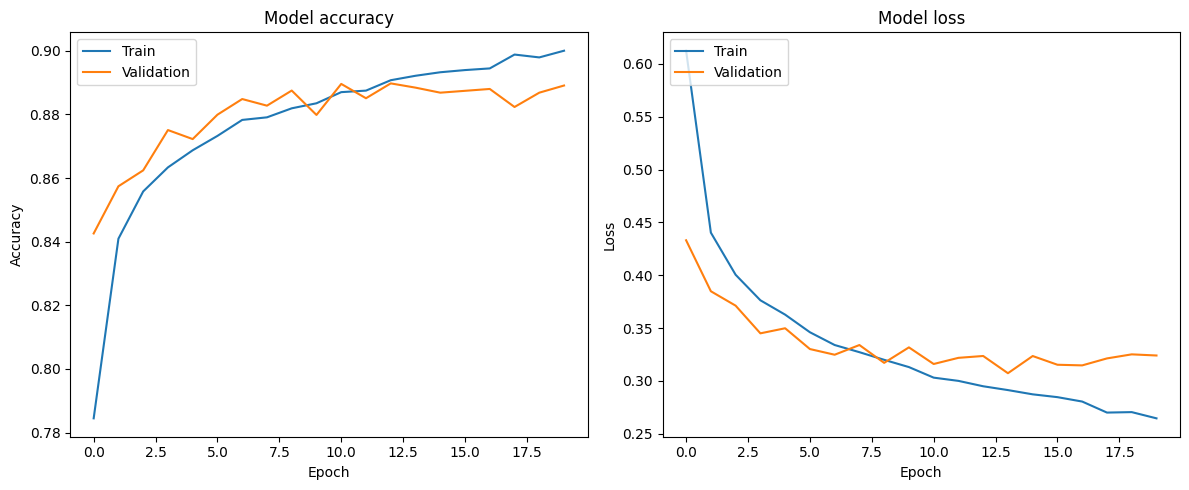
\includegraphics[width=0.8\textwidth]{5.png}
	\caption{多层感知机训练图}
\end{figure}

为了更详细地了解模型的性能,我们使用 \texttt{sklearn} 提供的 \texttt{classification\_report} 来生成分类报告。这个报告显示了每个类别的 \texttt{precision}、\texttt{recall} 和 \texttt{f1-score}:

\begin{lstlisting}[language=Python]
	print(classification_report(y_test, y_pred, target_names=[
	'T-shirt/top', 'Trouser', 'Pullover', 'Dress', 'Coat',
	'Sandal', 'Shirt', 'Sneaker', 'Bag', 'Ankle boot']))
\end{lstlisting}


混淆矩阵可以帮助我们了解模型在哪些类别上表现良好以及哪些类别上表现不佳。我们使用 \texttt{sklearn} 提供的 \texttt{confusion\_matrix} 来生成混淆矩阵,并使用 \texttt{seaborn} 来绘制热力图:

\begin{lstlisting}[language=Python]
	cm = confusion_matrix(y_test, y_pred)
	plt.figure(figsize=(10, 8))
	sns.heatmap(cm, annot=True, fmt='d', cmap='Blues', xticklabels=[
	'T-shirt/top', 'Trouser', 'Pullover', 'Dress', 'Coat',
	'Sandal', 'Shirt', 'Sneaker', 'Bag', 'Ankle boot'],
	yticklabels=[
	'T-shirt/top', 'Trouser', 'Pullover', 'Dress', 'Coat',
	'Sandal', 'Shirt', 'Sneaker', 'Bag', 'Ankle boot'])
	plt.xlabel('Predicted Label')
	plt.ylabel('True Label')
	plt.title('Confusion Matrix')
	plt.show()
\end{lstlisting}
\begin{figure}[htbp]
	\centering
	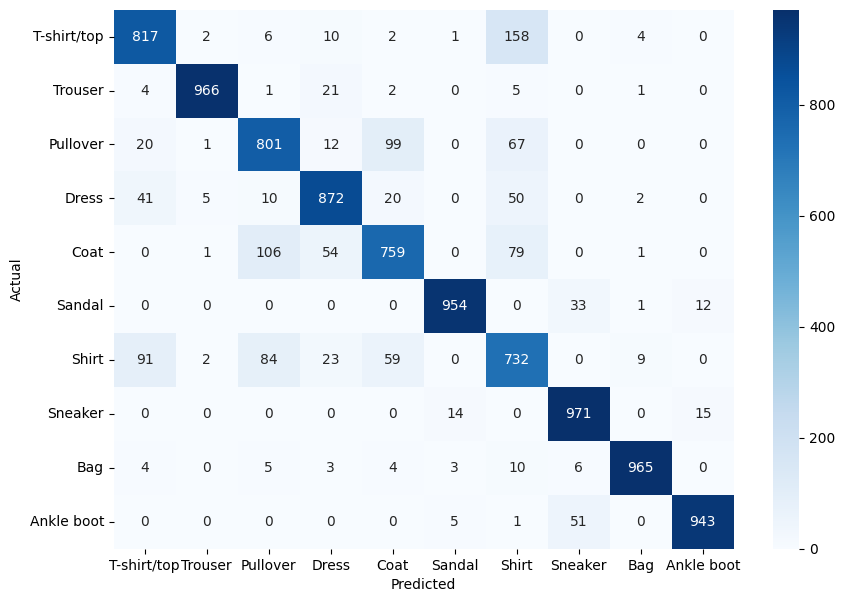
\includegraphics[width=0.8\textwidth]{6.png}
	\caption{多层感知机训练混淆矩阵}
\end{figure}

为了更直观地了解模型的预测效果,我们展示了前9个测试样本的真实标签和预测标签:

\begin{lstlisting}[language=Python]
	plt.figure(figsize=(10, 10))
	for i in range(9):
	plt.subplot(3, 3, i + 1)
	plt.imshow(x_test[i].reshape(28, 28), cmap='gray')
	plt.title(f"Pred: {y_pred[i]}, Actual: {y_test[i]}")
	plt.axis('off')
	plt.tight_layout()
	plt.show()
\end{lstlisting}


\begin{figure}[htbp]
	\centering
	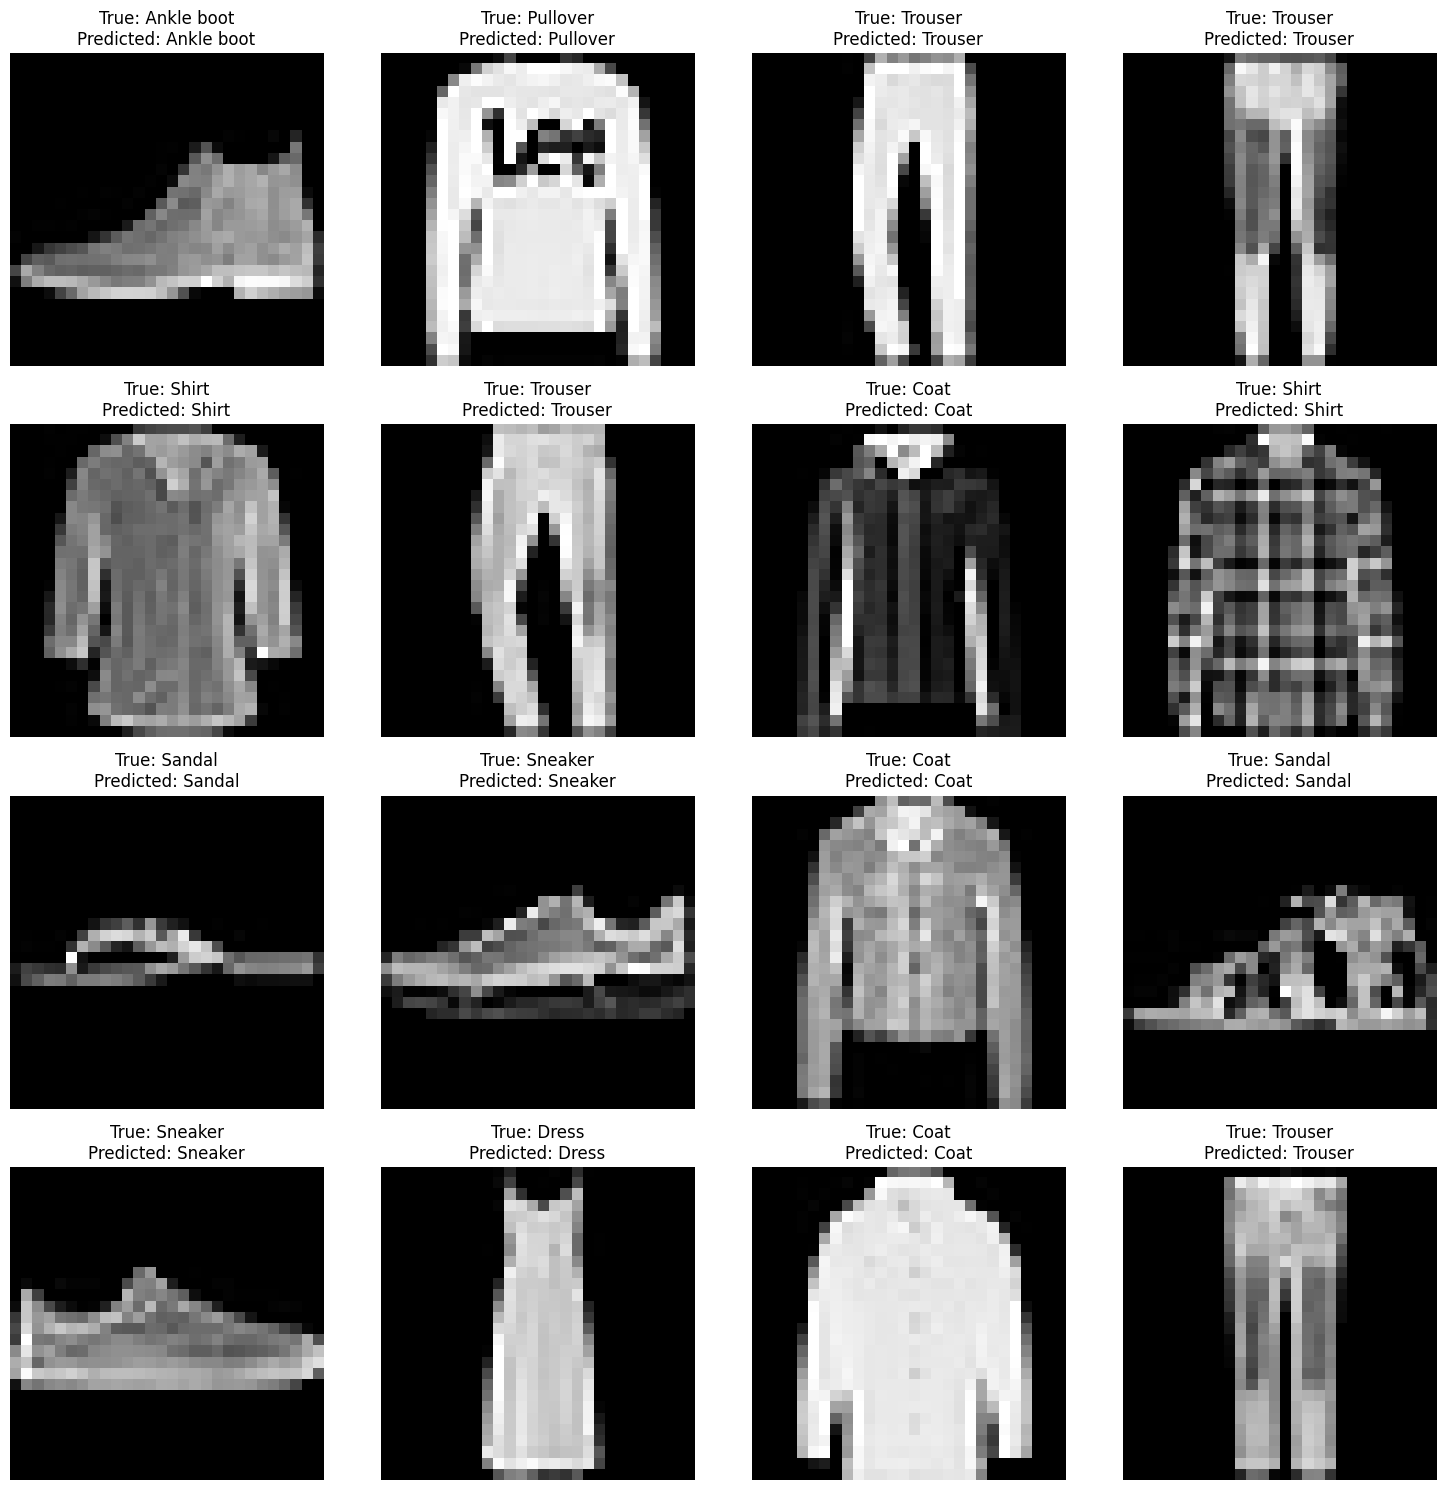
\includegraphics[width=0.6\textwidth]{7.png}
	\caption{多层感知机预测样例}
\end{figure}


\newpage
\section{Kaggle 房价预测}
\subsection{实验目的}
设计实现房价预测模型,在 kaggle 房价数据集上训练并验证性能。
\subsection{实验原理}
线性回归是统计学中最基础且广泛使用的预测模型之一,其基本假设是目标变量$y$与一组预测变量或特征$\mathbf{x}$之间存在线性关系。此模型的优势在于简单、易于实现,且可以给出关于数据关系的可解释性强的模型。

\subsection{模型描述}
线性回归模型试图找到一组权重$\mathbf{w}$和偏置$b$,使得模型的预测值$\hat{y}$与真实值$y$之间的差异最小。模型的数学表达式为:
\[
y = \mathbf{w}^\top \mathbf{x} + b
\]
展开形式为:
\[
y = w_1 x_1 + w_2 x_2 + \ldots + w_n x_n + b
\]
其中,$\mathbf{x} = [x_1, x_2, \ldots, x_n]^\top$是一个包含$n$个特征的向量,$\mathbf{w} = [w_1, w_2, \ldots, w_n]^\top$是对应特征的权重向量,$b$是模型的偏置项。

\subsection{模型假设}
线性回归模型基于以下几个关键假设:
\begin{enumerate}
	\item \textbf{线性关系:} 目标变量$y$与每个特征$x_i$之间应存在近似的线性关系。
	\item \textbf{同方差性:} 不同的观测值的误差项应具有相同的方差。
	\item \textbf{误差项的独立性:} 误差项之间应相互独立,即一个误差项的出现不应影响另一个误差项。
	\item \textbf{无多重共线性:} 特征之间不应该存在完全的线性关系,即特征矩阵应具有较高的秩。
\end{enumerate}

\subsection{优化目标}
模型训练的目标是最小化预测值$\hat{y}$与实际值$y$之间的差异,通常通过最小化一个损失函数来实现,最常用的是均方误差(MSE)损失函数:
\[
\text{MSE} = \frac{1}{N} \sum_{i=1}^{N} (y_i - \hat{y}_i)^2
\]
其中$N$是样本的总数,$y_i$是第$i$个样本的实际值,$\hat{y}_i$是模型对第$i$个样本的预测值。

通过优化这一目标,线性回归模型不仅能提供对数据的良好拟合,还能通过分析权重$\mathbf{w}$的值来理解各特征对目标变量的影响程度。





\subsection{数据预处理}
数据预处理是任何机器学习任务中的重要步骤,其目的是将原始数据转换成适合模型学习的格式。在本实验中,主要包括以下几个步骤:

\begin{enumerate}
	\item \textbf{标准化处理:} 标准化是调整数值型特征的尺度,使之符合标准正态分布,即平均值为0,标准差为1。这样做可以减少特征间尺度差异对模型的影响,特别是在使用基于梯度的优化算法时,可以加快收敛速度。标准化的数学表达式为:
	\[
	\mathbf{x}' = \frac{\mathbf{x} - \mu}{\sigma}
	\]
	其中$\mathbf{x}$是原始特征向量,$\mu$和$\sigma$分别是$\mathbf{x}$的均值和标准差。
	
	\item \textbf{缺失值处理:} 在数据集中常常存在缺失值,未处理的缺失值可能会导致模型训练过程中的错误。一种常见的处理方法是将缺失值填充为0,这种方法简单且不会引入额外的误差,但前提是0不会对数据的含义造成影响。数学上可以表示为:
	\[
	\mathbf{x}'_i = \begin{cases} 
		\mathbf{x}_i & \text{if } \mathbf{x}_i \text{ is not missing} \\
		0 & \text{if } \mathbf{x}_i \text{ is missing}
	\end{cases}
	\]
	
	\item \textbf{类别特征编码:} 对于类别特征,直接使用数值表示可能会误导模型认为其中包含数学上的顺序或大小关系,这对于那些没有实际数量意义的数据是不恰当的。因此,将类别特征转换为独热编码格式是解决此问题的有效方法。独热编码为每个类别属性创建一个新的布尔列,其中只有对应类别为1,其余为0。设类别特征$\mathbf{x}$有$m$个类别,转换后的特征$\mathbf{x}'$将是一个$m$维向量,其数学表达式为:
	\[
	\mathbf{x}' = \begin{cases} 
		1 & \text{if } \mathbf{x} = \text{category}_i \\
		0 & \text{otherwise}
	\end{cases}
	\]
\end{enumerate}


\subsection{优化算法:Adam算法}
在训练线性回归模型时,选择合适的优化算法是至关重要的。本实验中使用的Adam优化算法,是一种高效的随机梯度下降方法,适用于大规模数据和参数的优化。Adam结合了动量法和RMSProp算法的优点,通过计算梯度的一阶矩估计和二阶矩估计来调整每个参数的学习率。

\subsubsection{Adam算法原理}
Adam算法的更新规则基于对每个参数的一阶矩(均值)和二阶矩(未中心化的方差)的估计。具体数学表达如下:

\begin{enumerate}
	\item \textbf{计算梯度:} 首先计算损失函数关于参数$\theta$(在本实验中为$\mathbf{w}$和$b$)的梯度:
	\[
	g_t = \nabla_{\theta} L(\theta_t)
	\]
	其中$L$是损失函数,$g_t$是在时间步$t$的梯度。
	
	\item \textbf{更新一阶和二阶矩估计:} 使用指数加权平均估计梯度的一阶矩(均值)$m_t$和二阶矩(方差)$v_t$:
	\[
	m_t = \beta_1 m_{t-1} + (1 - \beta_1) g_t, \quad v_t = \beta_2 v_{t-1} + (1 - \beta_2) g_t^2
	\]
	其中$\beta_1$和$\beta_2$是衰减率,通常接近1。
	
	\item \textbf{偏差校正:} 由于$m_t$和$v_t$是初始化为0的,直接使用它们会导致估计偏向于0,特别是在迭代初期。因此,需要对它们进行偏差校正:
	\[
	\hat{m}_t = \frac{m_t}{1 - \beta_1^t}, \quad \hat{v}_t = \frac{v_t}{1 - \beta_2^t}
	\]
	
	\item \textbf{参数更新:} 最后,使用校正后的一阶矩和二阶矩来更新参数:
	\[
	\theta_{t+1} = \theta_t - \eta \frac{\hat{m}_t}{\sqrt{\hat{v}_t} + \epsilon}
	\]
	其中$\eta$是学习率,$\epsilon$是为了保持数值稳定性而添加的一个很小的常数(通常为$10^{-8}$)。
\end{enumerate}

Adam算法通过这种方式调整每个参数的学习率,使得参数更新更加稳健。这种自适应学习率的方法对于处理非均匀数据的更新有很大的优势,特别是在复杂的模型和大规模数据集上。


\subsection{交叉验证原理}
为了确保机器学习模型具有良好的泛化能力,即在新的、未见过的数据上也能表现出良好的预测性能,常常采用交叉验证(Cross-Validation)的方法来评估模型性能。$k$-折交叉验证是一种常见的交叉验证方法,它能够有效地利用有限的数据来获取模型在未知数据上表现的可靠估计。

\subsubsection{交叉验证的步骤}
$k$-折交叉验证的步骤可以描述如下:

\begin{enumerate}
	\item \textbf{数据分割:} 将全部训练数据随机分为$k$个大小大致相等的子集。每个子集尽可能保持数据的分布一致性,以确保验证的公正性。
	
	\item \textbf{模型训练与验证:} 依次选取其中一个子集作为验证集,剩余的$k-1$个子集合并作为训练集。对模型进行训练后,在当前的验证集上评估模型的性能。这一过程重复$k$次,每次选择不同的子集作为验证集。
	
	\item \textbf{性能评估:} 每一轮结束后,会得到一个性能指标(如误差率、准确率等),最后计算这$k$次性能指标的平均值,以此作为模型的综合性能指标。
\end{enumerate}

\subsubsection{数学表达}
设$\mathcal{D}$是整个数据集,将$\mathcal{D}$平均分成$k$个互不重叠的子集,记为$\mathcal{D}_1, \mathcal{D}_2, \ldots, \mathcal{D}_k$。对于每一次$i \in \{1, 2, \ldots, k\}$的迭代,设$\mathcal{D}_i$为验证集,其余的$\mathcal{D} \setminus \mathcal{D}_i$合并后作为训练集。定义模型在第$i$次迭代的验证结果为$E_i$,模型在$k$-折交叉验证中的平均性能可以表示为:
\[
E_{\text{avg}} = \frac{1}{k} \sum_{i=1}^k E_i
\]

\subsubsection{交叉验证的优点}
\begin{itemize}
	\item \textbf{泛化性能:} 通过多次在不同的训练集和验证集上评估模型,可以更准确地估计模型在新数据上的表现。
	\item \textbf{避免过拟合:} 由于每次都使用不同的数据集进行训练和测试,模型不太可能在特定的数据集上过度优化。
	\item \textbf{数据利用率高:} 相比单一的训练集/测试集划分,$k$-折交叉验证使得每个数据点都被用作了训练和验证,提高了数据的使用效率。
\end{itemize}

这种方法尤其适用于数据量不是很大的情况,可以有效避免数据划分导致的训练数据不足的问题。


\subsection{性能度量:对数均方根误差(RMSLE)}
在预测模型中,性能度量是评估模型预测准确性的重要方面。对于房价预测等涉及金融数额预测的任务,常常希望误差度量能更多地关注相对误差而非绝对误差,特别是在目标变量的范围较广时。对数均方根误差(RMSLE)是一个在这类情形下特别有用的性能度量。

\subsubsection{RMSLE的定义}
RMSLE专门用于衡量两个数的相对差异,其定义如下:
\[
\text{RMSLE} = \sqrt{\frac{1}{n} \sum_{i=1}^n (\log(\mathbf{y}_i + 1) - \log(\hat{\mathbf{y}}_i + 1))^2}
\]
其中,$n$ 是样本总数,$\mathbf{y}_i$ 是第$i$个实际值,$\hat{\mathbf{y}}_i$ 是第$i$个预测值。$\log$ 函数的加一操作确保了即使在$\mathbf{y}_i$或$\hat{\mathbf{y}}_i$为0时,其对数也是有定义的。

\subsubsection{RMSLE的特性}
\begin{itemize}
	\item \textbf{关注相对误差:} RMSLE 通过对目标变量和预测值取对数,将模型的评估重点放在预测误差的相对大小上,而不是绝对大小。这使得预测的10万与实际的10万1之间的误差与预测的100与实际的101之间的误差在量级上被视为相等。
	
	\item \textbf{对大误差的惩罚较小:} 相比于均方误差(MSE),RMSLE对大误差的惩罚较小,这对于某些应用场景来说是一个优点,因为它可以防止模型过度对极端值进行拟合。
	
	\item \textbf{促进预测精度的提高:} RMSLE更倾向于惩罚低估大值的情况,相比高估同等量级的小值。这种特性使得RMSLE非常适用于需要预测精度较高的金融领域和具有重尾分布的数据。
\end{itemize}

\subsubsection{RMSLE与其他度量的对比}
与均方误差(MSE)或均方根误差(RMSE)相比,RMSLE提供了不同的见解和优势。在处理具有极端值或当预测偏离真实值很远时,使用RMSLE可以提供更平衡的误差视图。这特别适用于数据具有指数增长或衰减特性的情况。

\subsection{实验过程}
使用前面的一些训练深度网络的基本工具和网络正则化的技术。通过 Kaggle 比赛,将所学知识付诸实践。同时有一些关于数据预处理、模型设计和超参数选择的内容。
\subsection{实验过程}
\subsubsection{概述}
本脚本使用PyTorch框架,实现了线性回归模型用于kaggle数据集预测房价。该脚本包括数据预处理、模型定义、训练、验证和测试几个主要部分。

\subsubsection{数据处理}
\begin{itemize}
	\item 加载训练和测试数据集。
	\item 合并数据集,统一进行数据预处理。
	\item 数值型特征标准化处理,填充缺失值。
	\item 将分类特征转换为虚拟变量。
	\item 将处理后的数据集转换为PyTorch张量。
\end{itemize}

\subsubsection{模型定义}
\begin{itemize}
	\item 定义了一个单层线性回归模型。
	\item 使用正态分布初始化模型参数。
\end{itemize}

\subsubsection{训练和验证}
\begin{itemize}
	\item 定义均方误差损失函数。
	\item 实现一个训练循环,包括前向传播、损失计算、反向传播和参数更新。
	\item 采用k折交叉验证方法评估模型性能。
	\item 通过半对数图展示训练和验证过程中的RMSE变化。
\end{itemize}

\subsubsection{测试和结果提交}
\begin{itemize}
	\item 在全部训练数据上训练模型。
	\item 对测试数据进行预测,生成提交文件。
\end{itemize}

\subsubsection{输出}
脚本输出每一折的训练和验证RMSE,以及平均RMSE。最终训练的RMSE以及预测结果被保存为CSV文件用于提交。
\subsection{结果展示}
\begin{lstlisting}[language=Python]
import torch
import torch.utils.data
from IPython import display
import torch.nn as nn
import numpy as np
import pandas as pd
import sys
import matplotlib.pyplot as plt
train_data = pd.read_csv("train.csv")
test_data = pd.read_csv("test.csv")

train_data.shape
test_data.shape

train_data.iloc[0:4, [0, 1, 2, 3, -3, -2, -1]]

all_features = pd.concat((train_data.iloc[:, 1:-1], test_data.iloc[:, 1:]))
numeric_features = all_features.dtypes[all_features.dtypes != 'object'].index
all_features[numeric_features] = all_features[numeric_features].apply(lambda x: (x - x.mean())/(x.std()))
all_features = all_features.fillna(0)
all_features = pd.get_dummies(all_features, dummy_na=True)
all_features.shape

bool_columns = all_features.select_dtypes(include='bool').columns
all_features[bool_columns] = all_features[bool_columns].astype(float)
print(all_features.dtypes)
n_train = train_data.shape[0]
train_features = torch.tensor(all_features[:n_train].values, dtype=torch.float32)
test_features = torch.tensor(all_features[n_train:].values, dtype=torch.float32)
train_labels = torch.tensor(train_data.SalePrice.values, dtype=torch.float32).view(-1, 1)

loss = torch.nn.MSELoss()

def get_net(feature_num):
	net = nn.Linear(feature_num, 1)
	for param in net.parameters():
		nn.init.normal_(param, mean=0, std=0.01)
	return net

def log_rmse(net, features, labels):
	with torch.no_grad():
		clipped_preds = torch.max(net(features), torch.tensor(1.0))
		rmse = torch.sqrt(2 * loss(clipped_preds.log(), labels.log()).mean())
	return rmse.item()
	
def train(net, train_features, train_labels, test_features, test_labels, num_epochs, 
		  learning_rate, weight_decay, batch_size):
	train_ls, test_ls = [], []
	dataset = torch.utils.data.TensorDataset(train_features, train_labels)
	train_iter = torch.utils.data.DataLoader(dataset, batch_size, shuffle=True)
	optimizer = torch.optim.Adam(params=net.parameters(), lr=learning_rate, weight_decay=weight_decay)
	net = net.float()
	for epoch in range(num_epochs):
		for X, y in train_iter:
			l = loss(net(X.float()), y.float())
			optimizer.zero_grad()
			l.backward()
			optimizer.step()
		train_ls.append(log_rmse(net, train_features, train_labels))
		if test_labels is not None:
			test_ls.append(log_rmse(net, test_features, test_labels))
		return train_ls, test_ls

def get_k_fold_data(k, i, X, y):
	assert k > 1
	fold_size = X.shape[0] // k
	X_train, y_train = None, None
	for j in range(k):
		idx = slice(j * fold_size, (j + 1) * fold_size)
		X_part, y_part = X[idx, :], y[idx]
		if j == i:
			X_valid, y_valid = X_part, y_part
		elif X_train is None:
			X_train, y_train = X_part, y_part
		else:
			X_train = torch.cat((X_train, X_part), dim=0)
			y_train = torch.cat((y_train, y_part), dim=0)
	return X_train, y_train, X_valid, y_valid
	
def use_svg_display():
	display.set_matplotlib_formats('svg')
	
def set_figsize(figsize=(3.5, 2.5)):
	use_svg_display()
	plt.rcParams['figure.figsize'] = figsize
	
def semilogy(x_vals, y_vals, x_label, y_label, x2_vals=None, y2_vals=None, 
			 legend=None, figsize=(3.5, 2.5)):
	set_figsize(figsize)
	plt.xlabel(x_label)
	plt.ylabel(y_label)
	plt.semilogy(x_vals, y_vals)
	if x2_vals and y2_vals:
		plt.semilogy(x2_vals, y2_vals, linestyle=':')
		plt.legend(legend)
	plt.show()
	
def k_fold(k, X_train, y_train, num_epochs, learning_rate, weight_decay, batch_size):
	train_l_sum, valid_l_sum = 0, 0
	for i in range(k):
		data = get_k_fold_data(k, i, X_train, y_train)
		net = get_net(X_train.shape[1])
		train_ls, valid_ls = train(net, *data, num_epochs, learning_rate, weight_decay, batch_size)
		train_l_sum += train_ls[-1]
		valid_l_sum += valid_ls[-1]
		if i == 0:
			semilogy(range(1, num_epochs + 1), train_ls, 'epochs', 'rmse', 
					 range(1, num_epochs + 1), valid_ls, ['train', 'valid'])
		print('flod %d, train rmse %f, valid rmse %f' % (i, train_ls[-1], valid_ls[-1]))
	return train_l_sum / k, valid_l_sum / k

k, num_epochs, lr, weight_decay, batch_size = 5, 100, 5, 0, 64
train_l, valid_l = k_fold(k, train_features, train_labels, num_epochs, lr, weight_decay, batch_size)
print('%d-fold validation: avg train rmse %f, avg valid rmse %f'%(k, train_l, valid_l))

def train_and_pred(train_features, test_features, train_labels, test_data, 
					num_epochs, lr, weight_decay, batch_size):
	net = get_net(train_features.shape[1])
	train_ls, _ = train(net, train_features, train_labels, None, None, num_epochs,
						lr, weight_decay, batch_size)
	semilogy(range(1, num_epochs+1), train_ls, 'epochs', 'rmse')
	print('train rmse %f'%train_ls[-1])
	preds = net(test_features).detach().numpy()
	test_data['SalePrice'] = pd.Series(preds.reshape(1, -1)[0])
	submission = pd.concat([test_data['Id'], test_data['SalePrice']], axis=1)
	submission.to_csv("./submission.csv", index=False)
	
train_and_pred(train_features, test_features, train_labels, test_data, num_epochs, lr, 
				weight_decay, batch_size)
\end{lstlisting}
\begin{figure}[htbp]
	\centering
	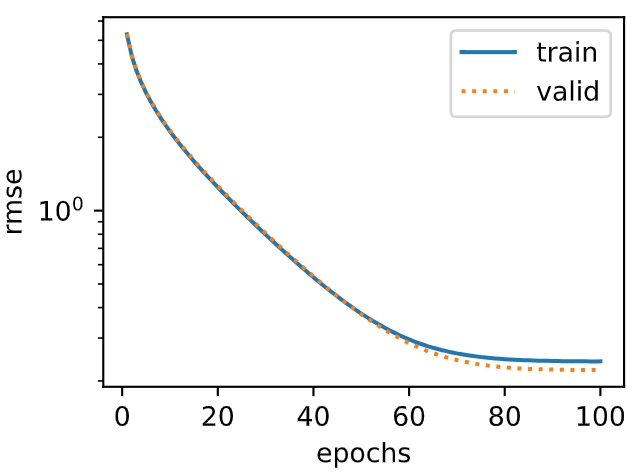
\includegraphics[width=0.8\textwidth]{18.png}
	\caption{线性回归训练结果}
\end{figure}

\begin{table}[h]
	\centering
	\caption{5-fold validation RMSE values}
	\label{tab:rmse_values}
	\begin{tabular}{|c|c|c|}
		\hline
		\textbf{Fold} & \textbf{Train RMSE} & \textbf{Valid RMSE} \\ \hline
		0 & 0.240618 & 0.222078 \\ \hline
		1 & 0.229766 & 0.267559 \\ \hline
		2 & 0.231669 & 0.238476 \\ \hline
		3 & 0.237572 & 0.218652 \\ \hline
		4 & 0.230357 & 0.258385 \\ \hline
		\textbf{Average} & \textbf{0.233997} & \textbf{0.241030} \\ \hline
	\end{tabular}
\end{table}

\begin{figure}[htbp]
	\centering
	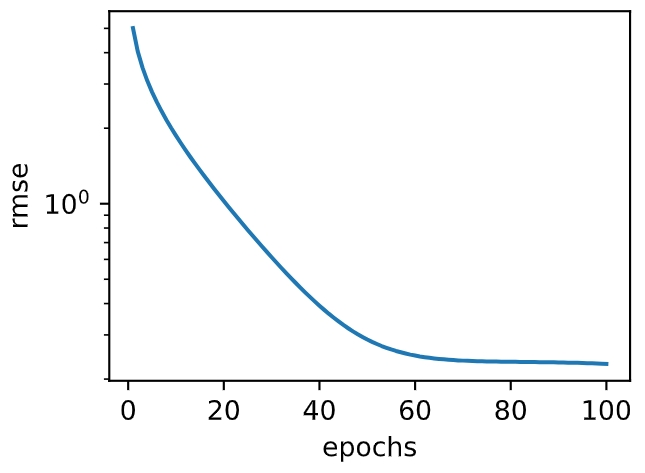
\includegraphics[width=0.8\textwidth]{19.png}
	\caption{线性回归训练预测结果}
\end{figure}

train rmse 0.229716

\newpage
\section{边缘检测}
\subsection{实验目的}
本实验旨在通过应用不同的卷积核来检测图像中的边缘,借此我们可深入了解图像处理中的边缘检测技术,掌握使用卷积核进行图像边缘提取的方法。实验中将使用如下几种卷积核:

\begin{itemize}
	\item 水平边缘检测卷积核:强调图像中水平方向的像素变化。
	\item 垂直边缘检测卷积核:强调图像中垂直方向的像素变化。
	\item 对角线边缘检测卷积核:强调图像中对角线方向的像素变化。
\end{itemize}

\subsection{实验原理}
在计算机视觉和图像处理领域,边缘检测是一种基本而重要的技术,用于识别图像中对象的边界。边缘通常被定义为图像亮度的显著变化,而边缘检测的目的是找到这些亮度显著变化的位置。

\subsubsection{数学基础}
边缘检测主要通过卷积操作实现,卷积操作是一种数学运算,它将卷积核(滤波器)应用于图像的每个像素,通过与核周围的像素值的加权和来更新当前像素的值。这一过程可用如下的数学表达式描述:
\begin{equation}
	I'(x, y) = \sum_{i=-k}^{k} \sum_{j=-k}^{k} K(i, j) \cdot I(x-i, y-j)
\end{equation}
其中,$I(x, y)$ 表示原始图像在位置 $(x, y)$ 的像素值,$K$ 代表卷积核,$I'(x, y)$ 是卷积操作后在位置 $(x, y)$ 的新像素值,$k$ 是卷积核的半径。此公式中的卷积核 $K(i, j)$ 与图像 $I(x-i, y-j)$ 的对应元素相乘,然后对所有乘积求和,得到的结果就是新图像在 $(x, y)$ 位置的像素值。


\subsubsection{卷积核设计}
边缘检测的核心在于使用特定设计的卷积核来识别图像中的边缘。本实验采用三种不同的卷积核来分别检测水平、垂直和对角线边缘,其设计原理如下:
\begin{itemize}
	\item \textbf{水平边缘检测卷积核}:
	此卷积核强调图像中水平方向的像素强度变化,适用于检测水平边缘。其数学表达式为:
	\begin{equation}
		K_h = \begin{bmatrix}
			-1 & -1 & -1 \\
			0 &  0 &  0 \\
			1 &  1 &  1
		\end{bmatrix}
	\end{equation}
	该核通过对水平相邻像素的高正负对比强调水平方向的灰度梯度。
	
	\item \textbf{垂直边缘检测卷积核}:
	此卷积核用于突出图像中垂直方向的像素强度变化,适合检测垂直边缘。其结构如下:
	\begin{equation}
		K_v = \begin{bmatrix}
			-1 & 0 & 1 \\
			-1 & 0 & 1 \\
			-1 & 0 & 1
		\end{bmatrix}
	\end{equation}
	该设计利用核中心列两侧的对称性差异来加强垂直边缘的视觉效果。
	
	\item \textbf{对角线边缘检测卷积核}:
	对角线卷积核用于检测图像中的对角线边缘,尤其是从左上到右下的方向。其形式为:
	\begin{equation}
		K_d = \begin{bmatrix}
			-1 & -1 & 2 \\
			-1 &  2 & -1 \\
			2 & -1 & -1
		\end{bmatrix}
	\end{equation}
	此卷积核通过强化特定对角线方向上的像素变化,从而有效地揭示该方向的边缘特征。
\end{itemize}

这些卷积核的设计考虑了图像中像素值变化的方向性,通过不同方向上的响应强度来强调和识别图像的边缘。通过精确调整卷积核参数,我们能够提高边缘检测的准确性和效果。

\subsection{结果展示}
\begin{lstlisting}[language=Python]
import cv2
import numpy as np
import matplotlib.pyplot as plt

def detect_edges(image_path):
	image = cv2.imread(image_path, cv2.IMREAD_GRAYSCALE)

	kernel_horizontal = np.array([[-1, -1, -1],
								[ 0,  0,  0],
								[ 1,  1,  1]])

	kernel_vertical = np.array([[-1, 0, 1],
								[-1, 0, 1],
								[-1, 0, 1]])

	kernel_diagonal = np.array([[-1, -1, 2],
								[-1, 2, -1],
								[ 2, -1, -1]])

	edges_horizontal = cv2.filter2D(image, -1, kernel_horizontal)
	edges_vertical = cv2.filter2D(image, -1, kernel_vertical)
	edges_diagonal = cv2.filter2D(image, -1, kernel_diagonal)

	plt.figure(figsize=(10, 8))
	plt.subplot(2, 2, 1)
	plt.imshow(image, cmap='gray')
	plt.title('Original Image')
	plt.axis('off')

	plt.subplot(2, 2, 2)
	plt.imshow(edges_horizontal, cmap='gray')
	plt.title('Horizontal Edges')
	plt.axis('off')

	plt.subplot(2, 2, 3)
	plt.imshow(edges_vertical, cmap='gray')
	plt.title('Vertical Edges')
	plt.axis('off')

	plt.subplot(2, 2, 4)
	plt.imshow(edges_diagonal, cmap='gray')
	plt.title('Diagonal Edges')
	plt.axis('off')

	plt.tight_layout()
	plt.show()

detect_edges("1.jpg")
\end{lstlisting}
\begin{figure}[htbp]
	\centering
	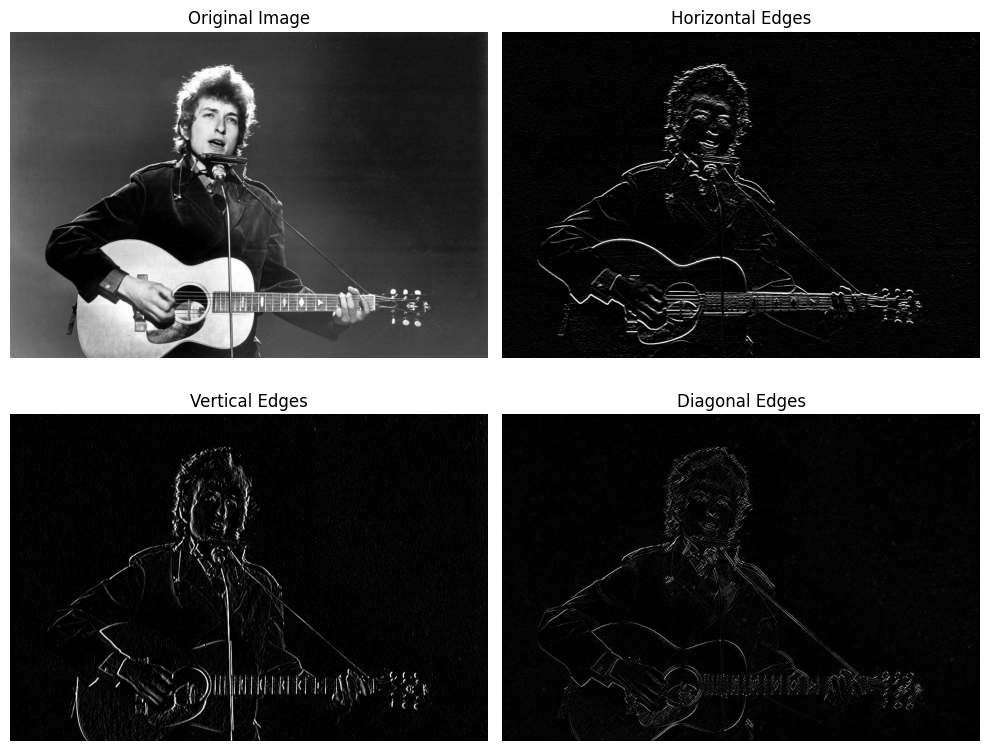
\includegraphics[width=1\textwidth]{8.png}
	\caption{不同边缘检测结果图}
\end{figure}


\newpage
\section{卷积输出形状的计算与验证}
\subsection{实验目的}
设计三组不同的填充和步幅组合,利用形状计算公式来计算输出形状,并实验
验证是否结果一致。
\subsection{实验原理}
本部分主要讨论卷积神经网络中卷积层输出形状的计算。卷积操作是图像处理中特征提取的核心操作。输出形状由输入形状、卷积核尺寸、填充和步长这几个参数决定。公式如下:
\[
H_{\text{out}} = \left\lfloor \frac{H_{\text{in}} + 2p - k}{s} + 1 \right\rfloor, \quad
W_{\text{out}} = \left\lfloor \frac{W_{\text{in}} + 2p - k}{s} + 1 \right\rfloor
\]
其中 \( H_{\text{in}} \) 和 \( W_{\text{in}} \) 分别表示输入的高度和宽度,\( p \) 表示填充量,\( s \) 表示步长,\( k \) 表示卷积核的尺寸。

\subsection*{参数影响解析}
\paragraph{填充 \( p \)} 填充是在输入数据的边界周围增加额外的、值通常为零的像素,用以控制输出数据的空间维度。填充的增加通常用于保持数据的尺寸,使得深层网络中信息能更深入地传递。
\paragraph{步长 \( s \)} 步长决定了卷积核滑动过程中的跳跃间隔。较大的步长会减小输出的空间维度,这有助于增加感受野,同时减少计算量。
\paragraph{卷积核尺寸 \( k \)} 卷积核的大小影响了每次卷积操作覆盖的区域大小,较大的卷积核可以捕获更宽广的特征,但同时也会增加计算负担。

\subsection*{具体计算实例}
我们考虑输入尺寸 \( H_{\text{in}} = W_{\text{in}} = 32 \) 和卷积核尺寸 \( k = 3 \),计算不同填充和步长组合下的输出形状:

\subsubsection*{情况一:\( p = 1 \),\( s = 1 \)}
使用一个单位的填充和一个单位的步长,输出尺寸保持不变:
\[
H_{\text{out}} = \left\lfloor \frac{32 + 2 \times 1 - 3}{1} + 1 \right\rfloor = 32, \quad
W_{\text{out}} = \left\lfloor \frac{32 + 2 \times 1 - 3}{1} + 1 \right\rfloor = 32
\]

\subsubsection*{情况二:\( p = 0 \),\( s = 2 \)}
不使用填充,并且步长为二,输出尺寸减半:
\[
H_{\text{out}} = \left\lfloor \frac{32 + 2 \times 0 - 3}{2} + 1 \right\rfloor = 15, \quad
W_{\text{out}} = \left\lfloor \frac{32 + 2 \times 0 - 3}{2} + 1 \right\rfloor = 15
\]

\subsubsection*{情况三:\( p = 2 \),\( s = 1 \)}
使用两个单位的填充和一个单位的步长,输出尺寸略有增加:
\[
H_{\text{out}} = \left\lfloor \frac{32 + 2 \times 2 - 3}{1} + 1 \right\rfloor = 34, \quad
W_{\text{out}} = \left\lfloor \frac{32 + 2 \times 2 - 3}{1} + 1 \right\rfloor = 34
\]


\subsection{结果展示}
\begin{lstlisting}[language=Python]
import torch
import torch.nn.functional as F
import matplotlib.pyplot as plt
import numpy as np

input_size = (1, 1, 32, 32)  # Format: (batch, channels, height, width)
kernel_size = 3

configurations = [
{"stride": 1, "padding": 1},
{"stride": 2, "padding": 0},
{"stride": 1, "padding": 2}
]

def calculate_output_size(H_in, W_in, padding, stride, kernel_size):
	H_out = ((H_in + 2 * padding - kernel_size) // stride) + 1
	W_out = ((W_in + 2 * padding - kernel_size) // stride) + 1
	return H_out, W_out

input_tensor = torch.randn(input_size)

results = []

for config in configurations:
	output_tensor = F.conv2d(input_tensor, 
							 weight=torch.randn(1, 1, kernel_size, kernel_size),
							 stride=config["stride"],
							 padding=config["padding"])
	output_shape = output_tensor.shape[2:]

	theoretical_output_shape = calculate_output_size(input_size[2], input_size[3], 
													 config["padding"], config["stride"], 
													 kernel_size)

	results.append({
		"config": f"Stride {config['stride']}, Padding {config['padding']}",
		"theoretical": theoretical_output_shape,
		"experimental": output_shape
	})

fig, ax = plt.subplots()
index = range(len(results))
bar_width = 0.35

theoretical_heights = [result["theoretical"][0] for result in results]
experimental_heights = [result["experimental"][0] for result in results]

rects1 = ax.bar(index, theoretical_heights, bar_width, label='Theoretical')
rects2 = ax.bar([p + bar_width for p in index], experimental_heights, bar_width, label='Experimental')

ax.set_xlabel('Configuration')
ax.set_ylabel('Output Heights')
ax.set_title('Comparison of Theoretical and Experimental Output Heights')
ax.set_xticks([p + bar_width / 2 for p in index])
ax.set_xticklabels([result["config"] for result in results])
ax.legend()

plt.show()

theoretical_sizes = np.array([list(result["theoretical"]) for result in results])
experimental_sizes = np.array([list(result["experimental"]) for result in results])
labels = [result["config"] for result in results]

fig, (ax1, ax2) = plt.subplots(1, 2, figsize=(12, 5))

heatmap1 = ax1.imshow(theoretical_sizes, cmap='viridis')
ax1.set_xticks(np.arange(2))
ax1.set_yticks(np.arange(len(labels)))
ax1.set_xticklabels(['Height', 'Width'])
ax1.set_yticklabels(labels)
ax1.set_title('Theoretical Output Sizes')
fig.colorbar(heatmap1, ax=ax1, orientation='vertical')

heatmap2 = ax2.imshow(experimental_sizes, cmap='viridis')
ax2.set_xticks(np.arange(2))
ax2.set_yticks(np.arange(len(labels)))
ax2.set_xticklabels(['Height', 'Width'])
ax2.set_yticklabels(labels)
ax2.set_title('Experimental Output Sizes')
fig.colorbar(heatmap2, ax=ax2, orientation='vertical')

plt.show()
\end{lstlisting}

\begin{figure}[htbp]
	\centering
	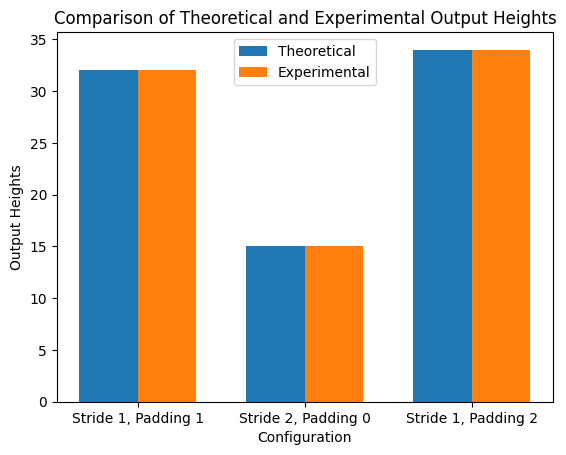
\includegraphics[width=0.5\textwidth]{9.png}
	\caption{理论实验对比柱形图}
\end{figure}

\begin{figure}[htbp]
\centering
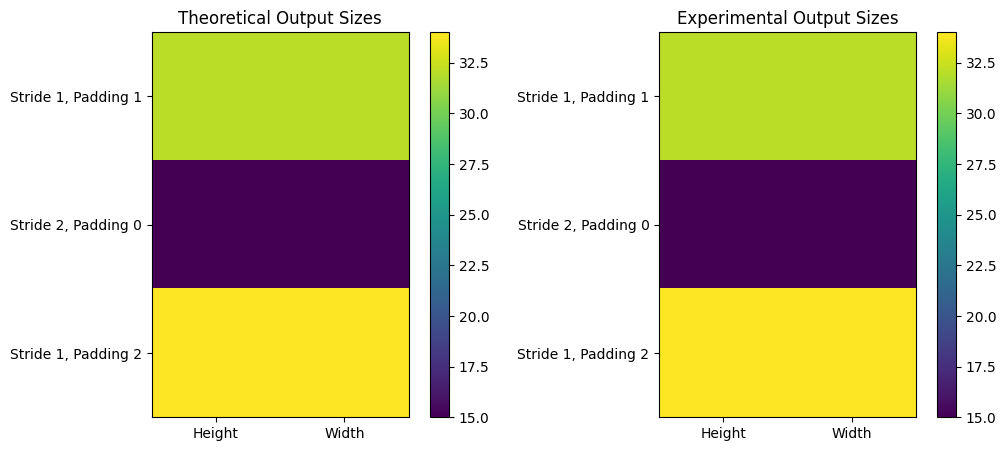
\includegraphics[width=0.7\textwidth]{10.png}
\caption{理论实验对比热力图}
\end{figure}
通过对不同参数设置下输出形状的计算,我们可以观察到填充和步长如何明显影响卷积层的输出维度。理解这些基本原理对于设计有效的卷积神经网络架构至关重要。

\newpage
\section{1*1 卷积核}
\subsection{实验目的}
利用 1*1 卷积核调整网络层之间的通道数,使得通道数减半。
\subsection{实验原理}
1x1卷积可以被视为在每个像素点上进行的独立的线性变换,这使得它能够在每个空间位置独立地转换输入特征。考虑输入特征图 \(X\),其中 \(X \in \mathbb{R}^{C_{\text{in}} \times H \times W}\),\(C_{\text{in}}\) 表示输入通道数,\(H\) 和 \(W\) 分别表示特征图的高度和宽度。

给定卷积核参数 \(W\) 和偏置 \(b\),1x1卷积的数学模型可以表示为:
\[
Y = W \cdot X + b
\]
这里,\(W \in \mathbb{R}^{C_{\text{out}} \times C_{\text{in}} \times 1 \times 1}\) 表示卷积核,其中 \(C_{\text{out}}\) 是输出通道数。\(b\) 是形状为 \(C_{\text{out}}\) 的偏置向量,每个输出通道有一个偏置值。

此操作可以理解为每个通道的输入被同一个 \(1 \times 1\) 的卷积核加权,然后按通道求和,最终产生新的输出通道。这种转换允许模型在不同通道间传递信息,有效地组合来自不同通道的信息,从而增强了模型对输入数据的表达能力。

在实验中,通过设置不同的输出通道数 \(C_{\text{out}}\),可以观察1x1卷积如何影响网络的学习能力和输出特征的表达。例如,增加 \(C_{\text{out}}\) 可以提高网络的容量,而减少 \(C_{\text{out}}\) 则有助于模型压缩和加速推理过程。

1x1卷积主要用于调整网络中的通道数,同时保持数据的空间维度(高度和宽度)不变。这种卷积操作对于特征整合和降维有着重要作用,在深层神经网络中用于增加网络的非线性能力和效率。

\subsection{结果展示}

通过实验验证,我们可以直接观察到不同配置下的输出特征图 \(Y\) 的变化,这些特征图展示了1x1卷积如何在实际应用中调整通道数和改变特征表达。结合可视化工具,如特征图的直方图或密度图,进一步揭示了1x1卷积操作的动态特性和影响。

\subsection{结果展示}
\begin{lstlisting}[language=Python]
import torch
import torch.nn as nn
import matplotlib.pyplot as plt
import seaborn as sns
input_channels = 8
output_channels = input_channels // 2  
input_size = (1, input_channels, 32, 32)  

input_tensor = torch.randn(input_size)

conv1x1 = nn.Conv2d(in_channels=input_channels, 
					out_channels=output_channels, 
					kernel_size=1, 
					stride=1, 
					padding=0)
output_tensor = conv1x1(input_tensor)

def plot_advanced_visualizations(tensor, title_prefix):
	tensor = tensor.detach() 
	fig, axes = plt.subplots(2, tensor.shape[1], figsize=(15, 6), sharex='col', gridspec_kw={'height_ratios': [1, 2]})

	for i in range(tensor.shape[1]):
		channel_data = tensor[0, i].flatten().numpy()

		sns.boxplot(x=channel_data, ax=axes[0, i], color='lightblue')
		axes[0, i].set_title(f'Channel {i+1} Box Plot')

		sns.kdeplot(channel_data, ax=axes[1, i], fill=True)
		axes[1, i].set_title(f'Channel {i+1} Density Plot')

	plt.suptitle(f'{title_prefix} Tensor Channels', fontsize=16, y=1.02)
	plt.tight_layout()
	plt.show()

	means = tensor.mean(dim=[0, 2, 3]).numpy()
	variances = tensor.var(dim=[0, 2, 3], unbiased=False).numpy()

	fig, (ax1, ax2) = plt.subplots(1, 2, figsize=(12, 4))

	ax1.plot(range(1, tensor.shape[1]+1), means, marker='o', linestyle='-', color='blue')
	ax1.set_title(f'{title_prefix} Channel Means')
	ax1.set_xlabel('Channel')
	ax1.set_ylabel('Mean')
	ax1.grid(True)

	ax2.plot(range(1, tensor.shape[1]+1), variances, marker='o', linestyle='-', color='red')
	ax2.set_title(f'{title_prefix} Channel Variances')
	ax2.set_xlabel('Channel')
	ax2.set_ylabel('Variance')
	ax2.grid(True)

	plt.suptitle(f'Means and Variances of {title_prefix} Tensor Channels', fontsize=16)
	plt.tight_layout()
	plt.show()

plot_advanced_visualizations(input_tensor, "Original")
plot_advanced_visualizations(output_tensor, "Output After 1x1 Convolution")
\end{lstlisting}

\begin{figure}[htbp]
	\centering
	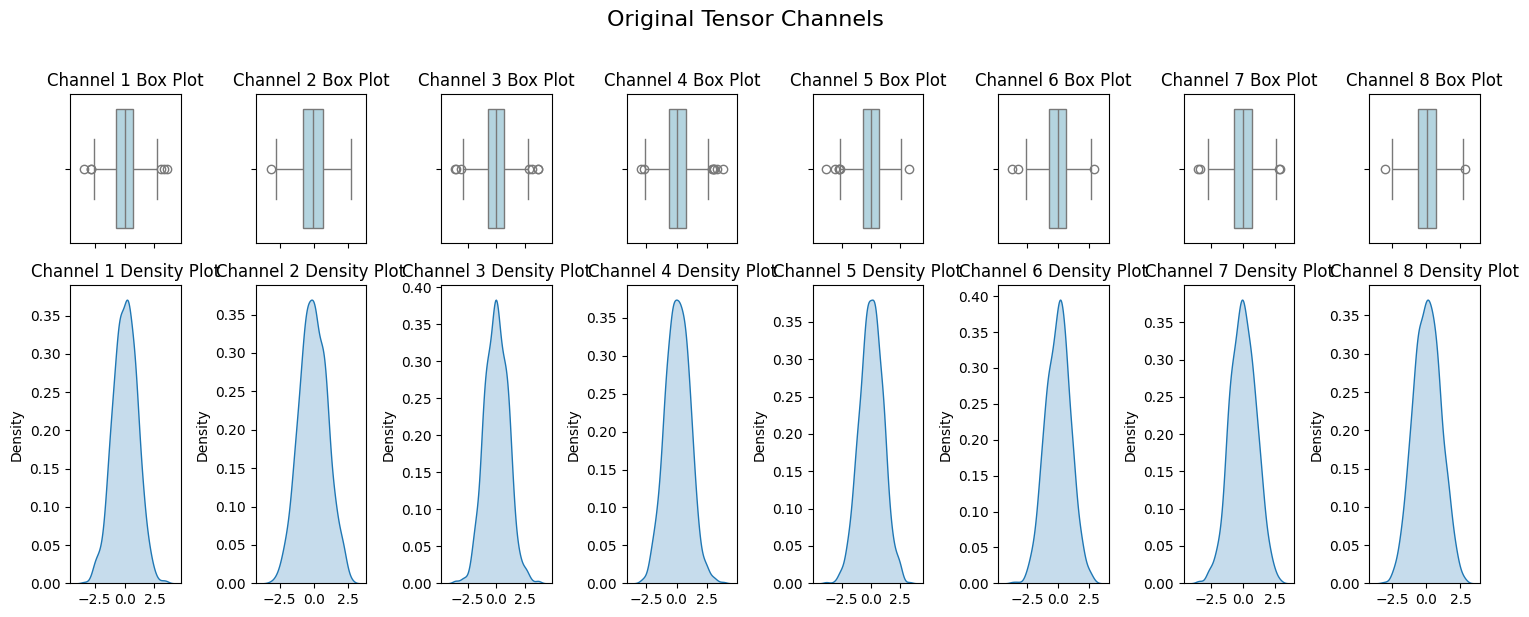
\includegraphics[width=1\textwidth]{13.png}
	\caption{原图 Tensor Channels}
\end{figure}

\begin{figure}[htbp]
	\centering
	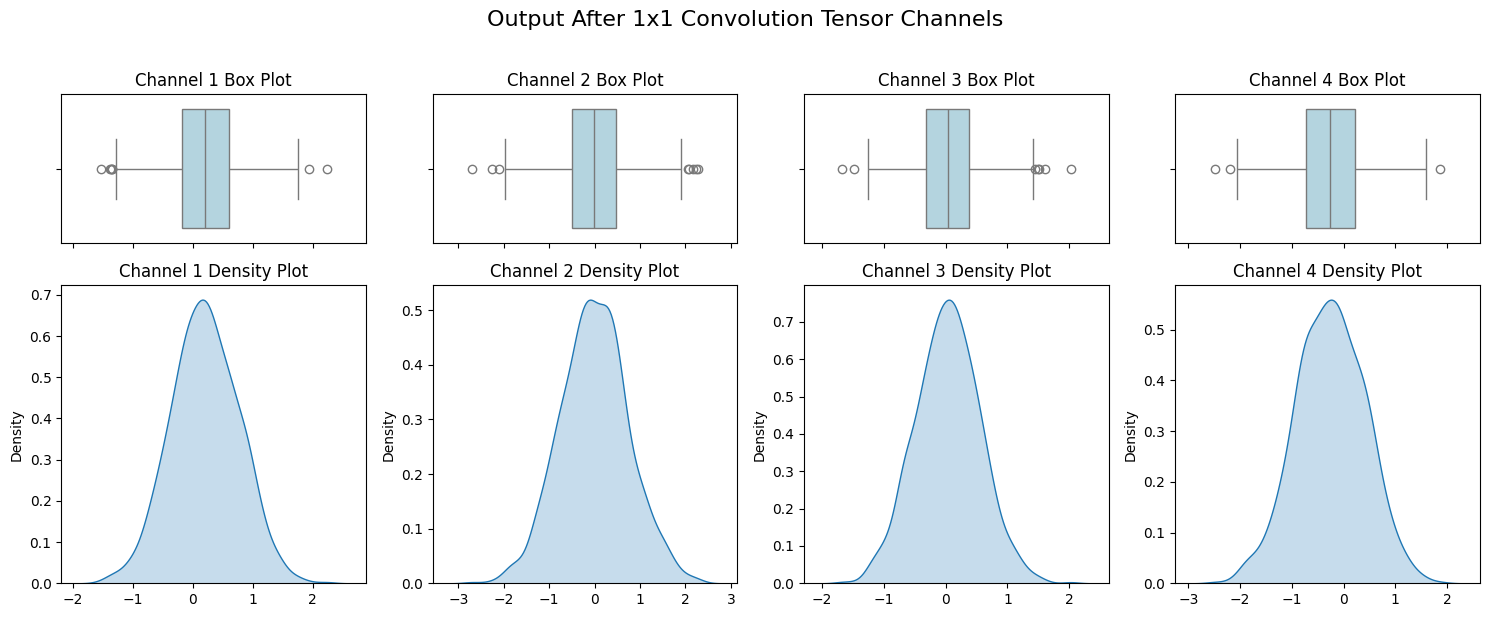
\includegraphics[width=1\textwidth]{15.png}
	\caption{1*1卷积后 Tensor Channels}
\end{figure}

\begin{figure}[htbp]
	\centering
	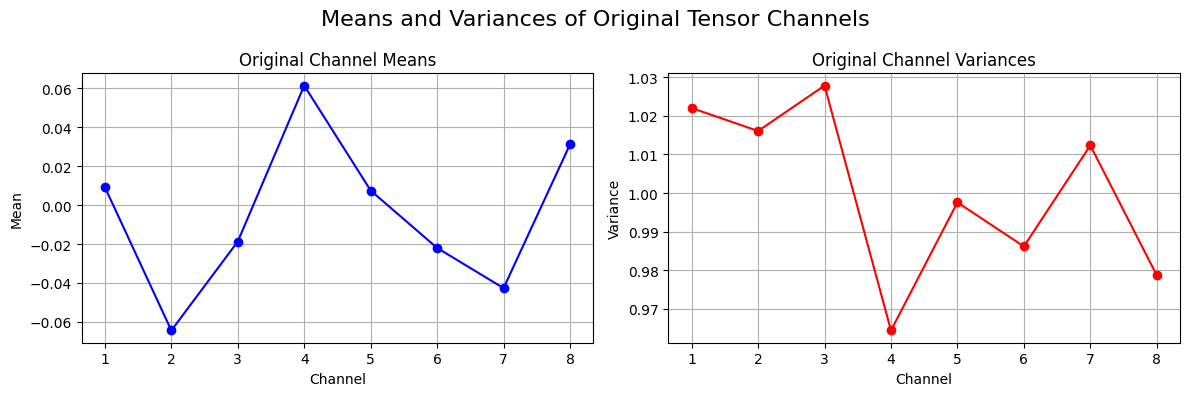
\includegraphics[width=0.7\textwidth]{14.png}
	\caption{原图 Tensor Channels}
\end{figure}
\begin{figure}[htbp]
	\centering
	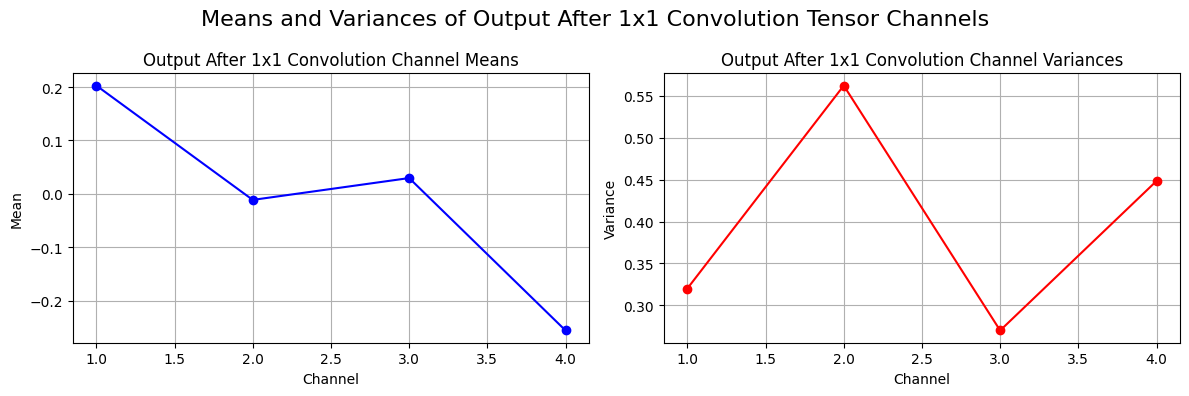
\includegraphics[width=0.7\textwidth]{16.png}
	\caption{1*1卷积后 Tensor Channels}
\end{figure}


\newpage
\section{LeNet}
\subsection{实验目的}
采用 LeNet 对 MNIST 数据库进行识别,测试不同卷积核大小、填充和步长
组合对结果的影响。
\subsection{实验原理}
本实验旨在探索卷积核尺寸、填充和步长参数在使用LeNet模型识别MNIST手写数字数据库时的影响。LeNet是早期卷积神经网络的经典结构之一,其设计主要针对图像识别任务。通过改变卷积层中的参数,我们可以评估这些变量对模型性能的影响。

\subsubsection{LeNet架构详解}
LeNet网络是一种早期的卷积神经网络,对现代深度学习框架中使用的许多网络架构有重要影响。LeNet主要用于图像识别任务,其结构设计优化了从原始图像数据中学习空间层级特征的能力。

\subsubsection*{卷积层的工作原理}
在LeNet架构中,卷积层承担着提取输入图像的空间特征的任务。这些层通过卷积运算有效地识别各种图像特征,如边缘、角点和其他纹理信息,这对于后续的图像识别任务至关重要。

\paragraph{卷积运算}
卷积层中的基本操作是卷积运算,该运算通过在输入图像上滑动卷积核(或滤波器),并在每个位置应用相同的权重集,从而提取特征。卷积操作可以用以下数学表达式精确描述:
\[
F_{ij}^{(l)} = \sigma\left(\sum_{m=-a}^{a}\sum_{n=-b}^{b} W_{mn}^{(l)} \cdot X_{(i+m)(j+n)} + b^{(l)}\right)
\]
其中,\( F_{ij}^{(l)} \) 代表第 \( l \) 层在位置 \( (i, j) \) 的输出特征值,\( W_{mn}^{(l)} \) 是卷积核中位于 \( (m, n) \) 位置的权重,\( X_{(i+m)(j+n)} \) 是输入特征图在相对位置 \( (i+m, j+n) \) 的像素值,\( b^{(l)} \) 是偏置项。这里,\( \sigma \) 表示激活函数,用于引入非线性,常见的激活函数包括ReLU和Sigmoid。

\paragraph{特征映射}
通过上述卷积运算,每个卷积核都能在输入图像上产生一个特征映射(Feature Map)。这个特征映射是原始输入数据的变换表示,突出显示了卷积核旨在检测的特定类型的特征。例如,某些卷积核可能专门用于检测边缘,而其他卷积核可能识别更复杂的图案如纹理或形状。

\paragraph{卷积层的作用}
卷积层的设计使得网络能够学习图像中的空间层级结构,这些结构随着网络的深入逐渐由简单到复杂。每一层的卷积核都会根据训练数据自动调整其权重,以最优方式响应图像中的特定特征,从而使得模型能够对新的、未见过的图像进行有效的分类和识别。


\subsubsection*{池化层的工作原理}
池化层主要功能是进行特征降维和保留关键信息。池化层通过对卷积层产生的特征映射进行下采样来实现这一点,有效地减少了数据的空间大小,从而减轻了计算负担,同时增加了模型对输入数据中小的变化和位移的鲁棒性。

\paragraph{池化操作的数学表达}
池化层可以采用不同的池化技术。最大池化操作通过选择覆盖区域中的最大值来进行下采样,而平均池化则计算区域中所有值的平均。这些操作可以通过以下数学表达式来描述:

\textbf{最大池化}:
\[
P_{ij}^{(l)} = \max_{a,b \in S}(F_{(i+a)(j+b)}^{(l)})
\]
\textbf{平均池化}:
\[
P_{ij}^{(l)} = \frac{1}{|S|}\sum_{a,b \in S} F_{(i+a)(j+b)}^{(l)}
\]
其中,\( P_{ij}^{(l)} \) 表示第 \( l \) 层池化后在位置 \( (i, j) \) 的输出值,\( S \) 是池化操作的窗口区域,\( F_{(i+a)(j+b)}^{(l)} \) 是池化窗口内相对于位置 \( (i, j) \) 的一个元素值,\( |S| \) 是窗口内元素的总数。

\paragraph{池化层的作用}
池化层的主要作用包括:
\begin{itemize}
	\item \textbf{控制过拟合}:通过减少参数的数量和模型的复杂性。
	\item \textbf{保持特征不变性}:帮助模型抵抗输入数据中的小的位置变化。
	\item \textbf{减少计算量}:降低特征维度后,随后的卷积层需要的计算量也相应减少。
\end{itemize}

池化层通过这些机制提高了网络的效率和性能,使得卷积神经网络能够更加有效地处理大规模和高维度的数据集。


\subsubsection*{全连接层的工作原理及其数学模型}
全连接层主要负责在特征提取完成后的信息合成与决策,通常位于网络的末端,用于将通过多个卷积和池化层处理后的高级特征映射转换为最终的输出。

\paragraph{数学表达}
全连接层的功能可以通过以下数学公式紧凑地表示:
\[
y_k = \sigma\left(\sum_{j} W_{jk} x_j + b_k\right)
\]
其中:
\begin{itemize}
	\item \( y_k \) 表示第 \( k \) 个输出神经元的激活值。
	\item \( W_{jk} \) 是连接第 \( j \) 个输入神经元和第 \( k \) 个输出神经元的权重。
	\item \( x_j \) 是来自上一层(可能是卷积层或池化层)的第 \( j \) 个神经元的输出。
	\item \( b_k \) 是第 \( k \) 个输出神经元的偏置项。
	\item \( \sigma \) 是激活函数,这可以是Sigmoid、Tanh或ReLU等,用于引入非线性,使得网络能够学习和模拟更复杂的函数。
\end{itemize}

\paragraph{全连接层的作用}
全连接层的主要作用是整合之前层次的学习到的特征,并做出最终的决策。由于全连接层的每个神经元都与前一层的所有神经元相连接,它能够学习输入数据中最有用的特征组合,以进行有效的预测或分类。这种层结构特别适用于那些需要基于全局信息进行决策的任务。

\paragraph{全连接层的参数量}
全连接层的参数量较大,是因为每个神经元都与前一层的所有神经元相连接。这种连接方式虽然提高了网络的学习能力,但同时也增加了模型的复杂度和计算量。因此,在设计深度学习模型时,应当合理安排全连接层的数量和大小,以平衡模型的性能和效率。


\subsubsection*{输出层}
最后,输出层通常包括一个softmax分类器,它将全连接层的输出转换为概率分布,表示输入图像属于各个类别的概率。
在深度学习网络中,输出层扮演着将网络的计算结果转换为可解释结果的关键角色。特别是在进行多类分类任务时,输出层通常采用softmax分类器来处理来自最后一个全连接层的信号。

\paragraph{Softmax函数的原理}
Softmax函数是一个逻辑函数,广泛用于多类分类问题中,将一个含任意实数的向量转换成一个实数向量,其元素值位于(0, 1)区间内,并且总和为1。因此,softmax函数的输出可以被视为一个概率分布。对于每一个输入样本,Softmax函数定义如下:
\[
\sigma(z)_j = \frac{e^{z_j}}{\sum_{k=1}^K e^{z_k}}
\]
其中,\( z \) 是来自上一全连接层的输入向量,\( K \) 是类别的总数,\( z_j \) 是向量 \( z \) 中的第 \( j \) 个元素,\( \sigma(z)_j \) 是该元素的softmax输出,代表了属于第 \( j \) 类的预测概率。

\paragraph{应用于输出层}
在神经网络中,特别是处理分类问题时,最后一个全连接层的输出会被送入softmax函数。这个过程可以表述为:
\[
\text{输出层概率} = \sigma(Wx + b)
\]
其中 \( W \) 表示权重矩阵,\( x \) 是从前一层传递来的特征向量,\( b \) 是偏置向量。通过应用softmax函数,网络能够输出每一个类别的预测概率,这些概率随后被用于计算损失函数,如交叉熵损失,进而指导模型训练过程。

\paragraph{交叉熵损失函数}
在训练分类模型时,常使用交叉熵损失函数来评估模型的预测结果与真实标签之间的差异。交叉熵损失函数的定义为:
\[
L = -\sum_{i=1}^N \sum_{j=1}^K y_{ij} \log(\hat{y}_{ij})
\]
其中,\( N \) 是样本数量,\( y_{ij} \) 是如果样本 \( i \) 属于类 \( j \) 则为1,否则为0的真实标签,\( \hat{y}_{ij} \) 是模型预测样本 \( i \) 属于类 \( j \) 的概率。

通过使用softmax函数和交叉熵损失,神经网络可以有效地学习多类数据的特征并进行准确的分类。

\subsubsection{卷积操作的数学表达}
给定输入特征图 \(X\),卷积操作可以表达为:
\[
Y = W \ast X + b
\]
其中 \(W\) 表示卷积核参数,\(b\) 表示偏置项,\(\ast\) 表示卷积操作,\(Y\) 是输出特征图。卷积核尺寸(\(k \times k\))、填充(\(p\))和步长(\(s\))是影响输出特征图大小和特性的关键参数。

\subsubsection{参数的影响}
\begin{itemize}
	\item \textbf{卷积核尺寸 \(k\)}: 较大的卷积核可以覆盖更广的输入区域,有助于捕获更大范围的特征,但可能会导致细节信息的丢失。
	\item \textbf{填充 \(p\)}: 填充用于控制输出的空间维度,增加填充可以使网络能够在边缘区域捕获更多信息。
	\item \textbf{步长 \(s\)}: 步长决定了卷积核滑动的间隔,较大的步长可以减小输出的空间尺寸,提高计算效率,但可能会降低模型的空间分辨率。
\end{itemize}

\subsubsection{实验设计}
本实验将通过对比不同的卷积核尺寸、填充和步长组合来评估它们对LeNet模型识别MNIST数据集性能的影响。我们将通过改变这些参数,观察模型在验证集上的精度和训练时间的变化,从而得出最佳的网络参数配置。实验涉及使用不同的核大小、填充和步长配置训练LeNet模型。每种配置都使用MNIST数据集进行训练,该数据集是一个广泛用于训练各种图像处理系统的大型手写数字数据库。MNIST数据集通过标准化转换进行准备,以标准化像素值。使用PyTorch的
DataLoader实用程序加载训练和测试数据集,该程序允许有效的批处理、洗牌和转换操作。该模型是LeNet架构的修改版本,适应于测试不同的卷积参数。网络由两个卷积层组成,后跟最大池化层,以及三个全连接层,最终输出分类结果。

实验包括测试四种不同的卷积层参数配置:
\begin{itemize}
	\item k = 3,p = 0,s = 1
	\item k = 5,p = 0,s = 1
	\item k = 5,p = 2,s = 1
	\item k = 3,p = 1,s = 2
\end{itemize}

每种配置训练10个周期,批量大小为64。模型使用Adam优化器和
CrossEntropyLoss作为损失函数进行训练。记录每个时期的训练损失,以监控学习进度。主要评估指标是测试数据集上的准确率,通过比较模型的预测与真实标签计算得出。训练后,将每种模型配置的准确率汇编成结果表,并绘制训练损失图表,以可视化和比较不同配置的学习动态。



\subsection{结果展示}
\begin{lstlisting}[language=Python]
import matplotlib.pyplot as plt
import numpy as np
import pandas as pd
import torch
import torch.nn as nn
import torch.optim as optim
import torchvision
import torchvision.transforms as transforms
from torch.utils.data import DataLoader

transform = transforms.Compose([transforms.ToTensor(), transforms.Normalize((0.5,), (0.5,))])
train_set = torchvision.datasets.MNIST(root='./data', train=True, download=True, transform=transform)
test_set = torchvision.datasets.MNIST(root='./data', train=False, download=True, transform=transform)
train_loader = DataLoader(train_set, batch_size=64, shuffle=True)
test_loader = DataLoader(test_set, batch_size=64, shuffle=False)

class LeNetVariant(nn.Module):
	def __init__(self, kernel_size=5, padding=0, stride=1, input_dim=28):
		super(LeNetVariant, self).__init__()
		self.conv1 = nn.Conv2d(1, 6, kernel_size=kernel_size, stride=stride, padding=padding)
		self.conv2 = nn.Conv2d(6, 16, kernel_size=kernel_size, stride=stride, padding=padding)
		self.pool = nn.MaxPool2d(2, 2)
		self.relu = nn.ReLU()

	def output_size(in_size):
		out_size = (in_size - (kernel_size - 1) - 1 + 2 * padding) // stride + 1
		out_size = (out_size - 2) // 2 + 1
		out_size = (out_size - (kernel_size - 1) - 1 + 2 * padding) // stride + 1
		out_size = (out_size - 2) // 2 + 1
		return out_size

	self.output_height = output_size(input_dim)
	self.output_width = output_size(input_dim)

	fc_input_features = 16 * self.output_height * self.output_width
	self.fc1 = nn.Linear(fc_input_features, 120)
	self.fc2 = nn.Linear(120, 84)
	self.fc3 = nn.Linear(84, 10)

	def forward(self, x):
		x = self.pool(self.relu(self.conv1(x)))
		x = self.pool(self.relu(self.conv2(x)))
		x = x.view(x.size(0), -1)
		x = self.relu(self.fc1(x))
		x = self.relu(self.fc2(x))
		x = self.fc3(x)
		return x
	def train_model(model, train_loader, test_loader, epochs=10):
		criterion = nn.CrossEntropyLoss()
		optimizer = optim.Adam(model.parameters())
		training_losses = []
		for epoch in range(epochs):
			model.train()
			total_loss = 0
			for i, data in enumerate(train_loader, 0):
				inputs, labels = data
				optimizer.zero_grad()
				outputs = model(inputs)
				loss = criterion(outputs, labels)
				loss.backward()
				optimizer.step()
				total_loss += loss.item()
			average_loss = total_loss / len(train_loader)
			training_losses.append(average_loss)
			print(f'Epoch {epoch + 1}, Loss: {average_loss:.4f}')
		test_accuracy = compute_accuracy(model, test_loader)
		print(f'Test Accuracy: {test_accuracy:.2f}%')
		return training_losses, test_accuracy

def compute_accuracy(model, data_loader):
	model.eval()
	correct = 0
	total = 0
	with torch.no_grad():
		for data in data_loader:
			images, labels = data
			outputs = model(images)
			_, predicted = torch.max(outputs.data, 1)
			total += labels.size(0)
			correct += (predicted == labels).sum().item()
	return 100 * correct / total

configurations = [
	{"kernel_size": 3, "padding": 0, "stride": 1},
	{"kernel_size": 5, "padding": 0, "stride": 1},
	{"kernel_size": 5, "padding": 2, "stride": 1},
	{"kernel_size": 3, "padding": 1, "stride": 2},
]

results = []
losses = []

for config in configurations:
	print(f'Training with kernel size: {config["kernel_size"]}, padding: {config["padding"]}, stride: {config["stride"]}')
	model = LeNetVariant(kernel_size=config["kernel_size"], padding=config["padding"], stride=config["stride"])
	training_losses, accuracy = train_model(model, train_loader, test_loader)
	results.append({"Configuration": f'KS={config["kernel_size"]}, P={config["padding"]}, S={config["stride"]}',
	"Accuracy": accuracy})
	losses.append(training_losses)

fig, ax = plt.subplots(1, 1, figsize=(14, 7))
for loss, config in zip(losses, configurations):
	ax.plot(loss, label=f'KS={config["kernel_size"]}, P={config["padding"]}, S={config["stride"]}')
ax.set_xlabel('Epoch')
ax.set_ylabel('Training Loss')
ax.set_title('Training Loss per Configuration')
ax.legend()

plt.show()

df_results = pd.DataFrame(results)
print(df_results)
\end{lstlisting}

\begin{figure}[htbp]
	\centering
	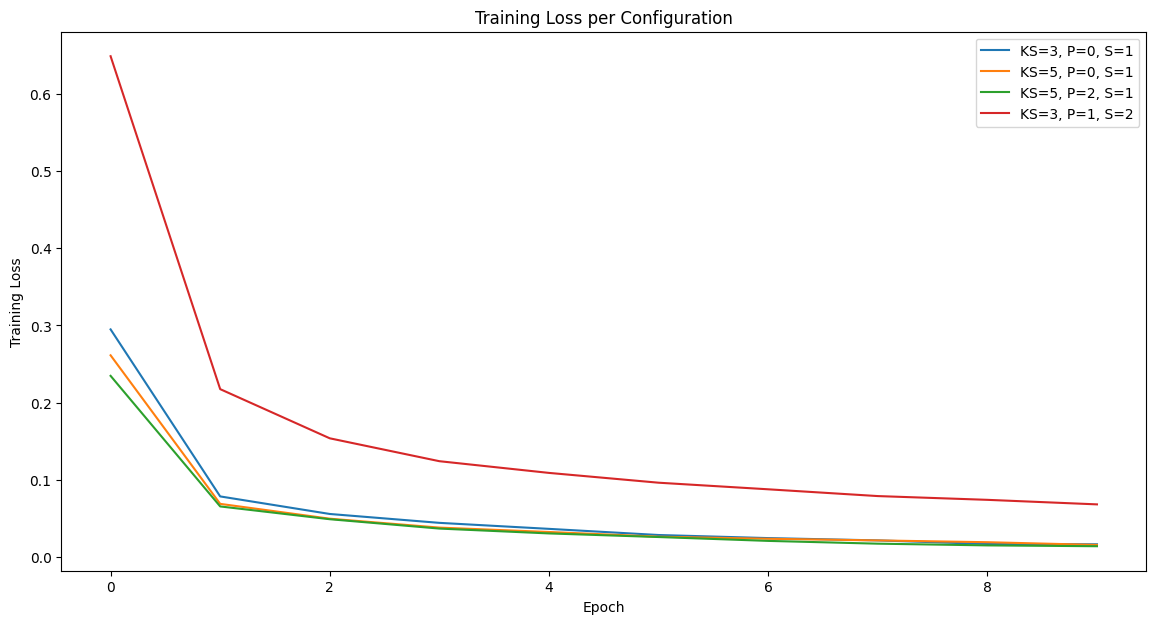
\includegraphics[width=1\textwidth]{17.png}
	\caption{不同配置下的训练图}
\end{figure}

\begin{table}[htbp]
	\centering
	\caption{不同配置下的模型和准确度}
	\begin{tabular}{@{}lc@{}}
		\toprule
		Configuration     & Accuracy (\%) \\ \midrule
		KS=3, P=0, S=1    & 98.76         \\
		KS=5, P=0, S=1    & 98.93         \\
		KS=5, P=2, S=1    & 99.09         \\
		KS=3, P=1, S=2    & 97.29         \\ \bottomrule
	\end{tabular}
\end{table}


\subsection{实验结论}
具有更大视野(通过更大的核或特定的填充/步长组合实现)的配置可能会捕获更多上下文信息,从而导致更高的准确率。


\newpage
\section{AlexNet}
\subsection{实验目的}
采用 AlexNet 对 MNIST 数据库进行识别,达到最优识别率。
\subsection{实验原理}
\subsection*{MNIST数据库简介}
MNIST数据库包含70000张手写数字图像,其中60000张用于训练,10000张用于测试。每张图像大小为$28 \times 28$像素,图像为灰度图。

AlexNet是一种深度卷积神经网络,具有强大的图像处理能力。本节将详细介绍使用AlexNet对MNIST数据库进行识别的原理和关键技术。

\subsubsection{网络结构}
AlexNet主要由五个卷积层和三个全连接层构成,具体结构如下:
\begin{itemize}
	\item 第一层:卷积层,使用$96$个大小为$11 \times 11$的卷积核,步长为$4$,后接最大池化。
	\item 第二层:卷积层,使用$256$个大小为$5 \times 5$的卷积核,包含重叠的最大池化。
	\item 第三层:卷积层,使用$384$个大小为$3 \times 3$的卷积核,不包括池化层。
	\item 第四层:同第三层。
	\item 第五层:卷积层,使用$256$个大小为$3 \times 3$的卷积核,后接最大池化。
	\item 三个全连接层:第一层和第二层各有$4096$个节点,最后一层根据需要调整节点数以适应不同的分类任务(对于MNIST,调整为$10$个节点)。
\end{itemize}

\subsubsection{前向传播和特征提取}
在AlexNet模型中,前向传播过程是实现图像识别的关键步骤,涉及卷积层、池化层和全连接层的协同工作。

\subsubsection*{卷积层}
卷积层的主要作用是提取输入图像的局部特征。卷积操作通过滑动窗口(卷积核)在输入图像上进行,以生成特征图。卷积核的每个元素与其覆盖的图像区域元素相乘后求和,从而实现特征提取。数学表示如下:
\begin{equation}
	f(x, y) = \sum_{i=-a}^{a} \sum_{j=-b}^{b} I(x-i, y-j) \cdot K(i, j)
\end{equation}
这里,$I$ 表示输入图像,$K$ 表示卷积核,$(i, j)$ 表示卷积核中的位置,$f(x, y)$ 表示得到的特征图的像素值。卷积层可以使用多个卷积核来提取不同的特征。

\subsubsection*{激活函数}
为了增加网络的非线性,每个卷积层后通常会跟一个激活函数,常用的激活函数是ReLU函数,其表达式为:
\begin{equation}
	g(z) = \max(0, z)
\end{equation}
其中$z$是卷积层输出的线性响应。ReLU函数能够有效地增加决策函数的非线性特性,并加速神经网络的训练过程。

\subsubsection*{池化层}
池化层位于连续的卷积层之间,用于降低特征维度和增强模型的泛化能力。池化操作通常采用最大池化,其取覆盖区域的最大值作为该区域的代表特征,数学上表示为:
\begin{equation}
	h(x, y) = \max_{(i, j) \in W} f(x+i, y+j)
\end{equation}
其中,$W$ 是池化窗口,$f(x+i, y+j)$ 是卷积层输出的特征图在窗口内的像素值。

\subsubsection*{全连接层}
经过多层的卷积和池化操作后,全连接层将所有特征合成,用于最终的分类。在全连接层中,来自前一层的所有特征被转化为一维向量,每个神经元都与前一层的所有神经元相连,输出可以通过softmax函数转化为概率形式,用于多类分类:
\begin{equation}
	p_k = \frac{e^{z_k}}{\sum_{j=1}^K e^{z_j}}
\end{equation}
其中,$z_k$ 是第$k$个输出神经元的输入,$p_k$ 是属于第$k$类的概率,$K$ 是类别总数。

这一系列操作确保了从原始图像到最终分类的决策的转化,使得AlexNet能够有效识别出不同类别的图像特征。


\subsubsection{反向传播和参数优化}
深度学习模型的训练核心是反向传播算法,它允许我们有效地计算网络中每个参数的梯度,进而通过梯度下降法更新这些参数以最小化损失函数。本部分详细解释这一过程及其在AlexNet训练中的应用。

\subsubsection*{损失函数}
在分类任务中,常用的损失函数是交叉熵损失函数,适用于多类分类问题。它测量的是模型预测概率分布与真实标签的分布之间的差异。数学表达式如下:
\begin{equation}
	L = -\sum_{i=1}^{C} y_i \log(p_i)
\end{equation}
其中,$C$ 表示类别总数,$y_i$ 是真实标签的独热编码(即如果样本属于类别$i$,则$y_i = 1$,否则为$0$),$p_i$ 是模型预测样本属于类别$i$的概率。

\subsubsection*{梯度计算}
反向传播算法首先计算损失函数关于网络输出的梯度,然后利用链式法则逐层向后传播这些梯度,直至输入层。对于每个参数,其梯度表示为损失函数对该参数的偏导数。对于权重$w_{ij}$,其梯度计算公式为:
\begin{equation}
	\frac{\partial L}{\partial w_{ij}} = \frac{\partial L}{\partial o_j} \cdot \frac{\partial o_j}{\partial w_{ij}}
\end{equation}
其中,$o_j$ 是该权重连接的神经元的输出。

\subsubsection*{参数更新}
在计算出所有相关梯度后,使用梯度下降法更新网络中的权重和偏置。权重更新规则为:
\begin{equation}
	w_{ij} \leftarrow w_{ij} - \eta \cdot \frac{\partial L}{\partial w_{ij}}
\end{equation}
其中,$\eta$ 是学习率,一个超参数,决定了在优化过程中参数更新的步长。

\subsubsection*{优化技术}
为了提高训练效率和模型性能,常见的优化技术包括动量(Momentum)、Adaptive Learning Rate(如Adam)等。这些方法调整学习率或在更新时考虑历史梯度,有助于加速收敛并减少训练过程中的震荡。

以上步骤重复进行,直至模型在验证集上的性能不再提高,或者达到预设的迭代次数。


\subsubsection{实验设置和优化}
在使用AlexNet对MNIST数据库进行识别的实验中,适当的数据预处理和优化策略是提高模型性能和泛化能力的关键。

\subsubsection*{数据预处理}
数据预处理是训练深度学习模型的第一步,主要包括以下几个方面:
\begin{itemize}
	\item \textbf{尺寸调整}:由于MNIST原始图像的大小为$28 \times 28$像素,而AlexNet需要$227 \times 227$像素的输入,因此必须对图像进行放缩处理。
	\item \textbf{归一化}:将图像像素值归一化到$[0, 1]$区间或标准化为均值为$0$,标准差为$1$的分布,可以加速模型收敛,并提高训练稳定性。归一化公式为:
	\begin{equation}
		I' = \frac{I - \mu}{\sigma}
	\end{equation}
	其中,$I$ 是原始图像,$\mu$ 和 $\sigma$ 分别是像素值的均值和标准差,$I'$ 是归一化后的图像。
\end{itemize}

\subsubsection*{数据增强}
数据增强是一种有效的方法来增加数据多样性,从而提高模型的泛化能力,尤其是在图像识别任务中。常用的数据增强技术包括:
\begin{itemize}
	\item 随机旋转
	\item 图像平移
	\item 缩放
	\item 水平翻转
\end{itemize}

\subsubsection*{Dropout和正则化}
为了防止模型过拟合,可以采用Dropout和L2正则化技术。Dropout通过随机丢弃一部分网络中的神经元,迫使网络学习更加鲁棒的特征。其数学表达式为:
\begin{equation}
	h' = h \cdot \text{Dropout}(p)
\end{equation}
其中,$h$ 是原始的神经元激活值,$p$ 是保留神经元的概率,$h'$ 是应用Dropout后的激活值。

L2正则化通过在损失函数中添加一个正则项来约束权重大小,减少模型复杂度,其正则化项为:
\begin{equation}
	L_{reg} = \lambda \sum_{w} w^2
\end{equation}
其中,$w$ 表示网络中的权重,$\lambda$ 是正则化强度参数。

这些策略共同作用,以优化网络训练过程,提高模型的泛化性能和准确率。
\subsection{实验过程}
本实验通过使用深度学习框架TensorFlow来实现一个基于AlexNet架构的卷积神经网络,目的是在MNIST手写数字数据集上进行图像识别。

\subsubsection{数据预处理}
实验首先加载MNIST数据集,该数据集包含手写数字的灰度图像。为了使这些图像适用于AlexNet,我们进行了以下预处理步骤:
\begin{itemize}
	\item 图像尺寸调整:将原始的$28 \times 28$像素图像调整为$224 \times 224$像素。
	\item 归一化处理:将图像像素值从整型转换为浮点型,并将其归一化到$[0, 1]$范围内。
	\item 颜色通道处理:由于AlexNet输入为彩色图像,我们通过复制单通道数据到三个通道,将灰度图转换为伪彩色图。
\end{itemize}

\subsubsection{模型构建}
使用TensorFlow和Keras构建AlexNet模型,其主要包含以下层:
\begin{itemize}
	\item 五个卷积层,用以提取图像特征。
	\item 三个最大池化层,用于降低特征的空间维度。
	\item 三个全连接层,最后一层采用softmax激活函数进行分类。
	\item Dropout层,防止过拟合。
\end{itemize}
模型的损失函数使用交叉熵,优化器选择Adam。

\subsubsection{训练与评估}
模型训练包括以下步骤:
\begin{itemize}
	\item 使用自定义的数据生成器,以批量方式提供训练和测试数据。
	\item 进行多个训练周期,每个周期包括对所有训练数据的一次前向传播和一次反向传播。
	\item 记录训练和验证过程中的准确率和损失值。
\end{itemize}
使用Matplotlib绘制训练和验证准确率及损失值的变化曲线,以可视化模型性能。


\subsection{结果展示}
\begin{lstlisting}[language=Python]
import tensorflow as tf
from tensorflow.keras import layers, models
from tensorflow.keras.datasets import mnist
from tensorflow.keras.utils import to_categorical, Sequence
import numpy as np
import matplotlib.pyplot as plt

class MNISTDataGenerator(Sequence):
	def __init__(self, images, labels, batch_size=32, shuffle=True):
		self.images = images
		self.labels = labels
		self.batch_size = batch_size
		self.shuffle = shuffle
		self.on_epoch_end()

	def __len__(self):
		return int(np.ceil(len(self.images) / self.batch_size))


	def __getitem__(self, index):
		batch_slice = slice(index * self.batch_size, (index + 1) * self.batch_size)
		x = self.images[batch_slice]
		y = self.labels[batch_slice]

		x = np.expand_dims(x, -1) 

		x_resized = np.array([tf.image.resize(img, (224, 224)).numpy() for img in x])
		x_resized = np.repeat(x_resized, 3, axis=3) 
		x_resized = x_resized.astype('float32') / 255.0

		return x_resized, y


	def on_epoch_end(self):
		if self.shuffle:
			indices = np.arange(len(self.images))
			np.random.shuffle(indices)
			self.images = self.images[indices]
			self.labels = self.labels[indices]

	def load_data():
		(train_images, train_labels), (test_images, test_labels) = mnist.load_data()
		train_labels = to_categorical(train_labels, 10)
		test_labels = to_categorical(test_labels, 10)
		return train_images, train_labels, test_images, test_labels

def build_alexnet_model(input_shape, num_classes):
	model = models.Sequential([
		layers.Conv2D(96, (11, 11), strides=4, activation='relu', input_shape=input_shape),
		layers.MaxPooling2D((3, 3), strides=2),
		layers.Conv2D(256, (5, 5), activation='relu', padding='same'),
		layers.MaxPooling2D((3, 3), strides=2),
		layers.Conv2D(384, (3, 3), activation='relu', padding='same'),
		layers.Conv2D(384, (3, 3), activation='relu', padding='same'),
		layers.Conv2D(256, (3, 3), activation='relu', padding='same'),
		layers.MaxPooling2D((3, 3), strides=2),
		layers.Flatten(),
		layers.Dense(4096, activation='relu'),
		layers.Dropout(0.5),
		layers.Dense(4096, activation='relu'),
		layers.Dropout(0.5),
		layers.Dense(num_classes, activation='softmax')
		])
		model.compile(optimizer='adam', loss='categorical_crossentropy', metrics=['accuracy'])
		return model

def plot_training_history(history):
	plt.figure(figsize=(12, 5))
	plt.subplot(1, 2, 1)
	plt.plot(history.history['accuracy'], label='Train Accuracy')
	plt.plot(history.history['val_accuracy'], label='Validation Accuracy')
	plt.title('Accuracy over Epochs')
	plt.xlabel('Epochs')
	plt.ylabel('Accuracy')
	plt.legend()

	plt.subplot(1, 2, 2)
	plt.plot(history.history['loss'], label='Train Loss')
	plt.plot(history.history['val_loss'], label='Validation Loss')
	plt.title('Loss over Epochs')
	plt.xlabel('Epochs')
	plt.ylabel('Loss')
	plt.legend()
	plt.show()

def main():
	train_images, train_labels, test_images, test_labels = load_data()
	train_gen = MNISTDataGenerator(train_images, train_labels, batch_size=64)
	test_gen = MNISTDataGenerator(test_images, test_labels, batch_size=64)

	model = build_alexnet_model((224, 224, 3), 10)
	history = model.fit(train_gen, validation_data=test_gen, epochs=10, verbose=2)
	plot_training_history(history)

if __name__ == "__main__":
	main()
\end{lstlisting}

\begin{figure}[htbp]
	\centering
	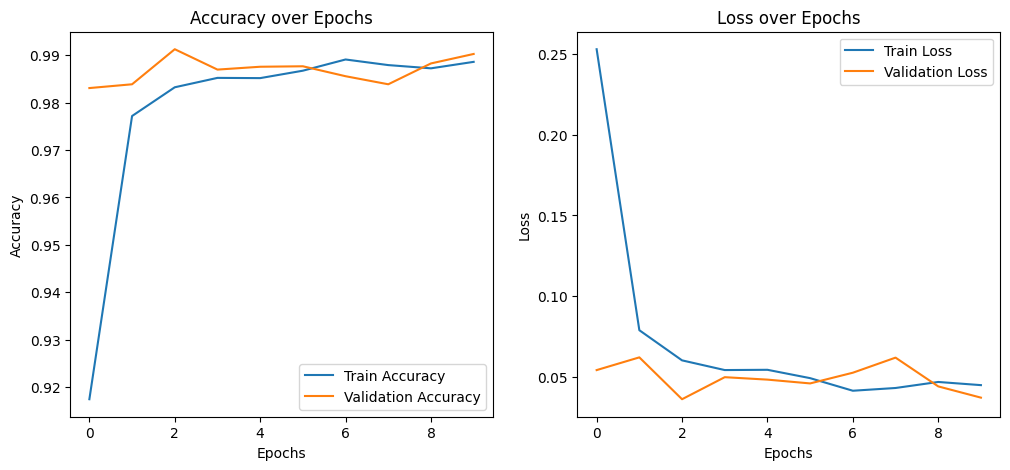
\includegraphics[width=1\textwidth]{20.png}
	\caption{不同配置下的训练图}
\end{figure}





\subsection{实验结论}
实验结果表明,通过适当的预处理和优化策略,AlexNet能够在MNIST数据集上实现高准确率的数字识别。图表展示了模型训练过程中准确率和损失值的变化,显示出模型随着训练周期增加而逐渐稳定和提高的性能。



\end{document}